\documentclass{iopjournal}

% IOPP / IOP Journal article class
% The class file (iopjournal.cls) and any required .bst bibliography styles
% should be uploaded to the Overleaf project root before compiling.

\begin{document}

\articletype{Paper}

\title{Spatio--Temporal Predictive Modelling of PM$_{2.5}$ in Karachi
from Multi-Source Satellite, Meteorological and Ground Observations
(2019--2023)}

\author{Sidhart Sami\orcid{0009-0003-8133-1230}}

\affil{Department of Computer Science, FAST National University of
Computer and Emerging Sciences, Karachi, Pakistan}

\email{sidhart.samir.punjabi@gmail.com}

\keywords{PM$_{2.5}$, air quality, machine learning, random forest,
long short-term memory, SHAP, Moran's I, LISA, digital twin, Karachi,
MERRA-2, MODIS, OpenAQ}

\begin{abstract}
Karachi's ambient PM$_{2.5}$ concentrations average approximately
12.3 times the World Health Organization 2021 annual guideline of
5\,\textmu g\,m$^{-3}$ on the 2019--2023 dataset analysed in this
study, placing it among the most polluted megacities in South Asia.
Systematic, data-driven characterisation of the city's pollution
sources and temporal structure remains limited in the peer-reviewed
literature. We address this gap by constructing a five-year daily
spatio-temporal dataset from eight ground monitoring stations fused
with multi-source satellite retrievals (Sentinel-5P trace gases,
MODIS MAIAC aerosol optical depth, ERA5 meteorological reanalysis,
VIIRS nighttime lights) and a strict ground-truth provenance chain
that combines OpenAQ per-station observations, a US Consulate
reference sensor, and MERRA-2 citywide surface PM$_{2.5}$. The final
modelling set contains 14\,400 station-day observations across 13
feature columns. We trained five traditional machine-learning models
and a unidirectional causal LSTM with self-attention on a 2019--2022
training set, evaluated on a held-out 2023 test set that the models
never saw. Random Forest achieved the best predictive performance
(RMSE\,=\,16.30\,\textmu g\,m$^{-3}$, MAE\,=\,10.63\,\textmu g\,m$^{-3}$,
R$^{2}$\,=\,0.612). The LSTM, despite approximately 480\,000 trainable
parameters and a 14-day lookback, produced a negative R$^{2}$ of
$-$0.104 on the test set, a result we interpret as evidence of a
fundamental data-density mismatch between complex sequence
architectures and eight monitoring stations. SHAP analysis of the
Random Forest identified \texttt{pm25\_lag1} and
\texttt{Optical\_Depth\_055} as the dominant predictors, indicating
that pollution persistence and aerosol loading explain most of the
predictable variance. Moran's I on the RF residuals is $-$0.19
($p$\,=\,0.28, not significant), confirming that no detectable
spatial autocorrelation remains after the RF absorbs the satellite
and meteorological features --- a positive finding about the model's
explanatory power rather than a defect. We release the full
preprocessing pipeline, processed dataset, trained model weights,
and an interactive 3D digital twin as an open-source repository
intended to be reusable for other data-sparse South Asian cities.
\end{abstract}

%-----------------------------------------------------------------------
\section{Introduction}
%-----------------------------------------------------------------------

\subsection{The Karachi air quality context}

Air pollution remains one of the leading contributors to the global
burden of disease. The Global Burden of Disease 2019 attributed
approximately 6.7 million deaths to ambient and household air
pollution combined \cite{GBD2019}, and the burden falls
disproportionately on South and East Asian cities where industrial
growth has outpaced regulatory enforcement. In South Asia, the
Indo-Gangetic Plain cities --- Delhi, Lahore, Dhaka --- receive the
most research attention. Karachi, Pakistan's commercial capital and
largest city, is discussed far less in the peer-reviewed literature,
yet its exposure levels are comparable to the most polluted cities in
the region.

Karachi is home to an estimated 16--20 million people. It hosts
Pakistan's largest port and industrial base, including steel mills,
petrochemical plants, textile factories, and power-generation units
concentrated in its northern and western industrial zones. The city's
meteorology compounds the problem: surrounded on the south by the
Arabian Sea but hemmed inland by flat terrain, Karachi experiences
persistent atmospheric inversions in winter months that trap
ground-level emissions. The annual average PM$_{2.5}$ concentration
on the eight-station dataset used in this study is approximately
61\,\textmu g\,m$^{-3}$, compared to the WHO 2021 annual guideline of
5\,\textmu g\,m$^{-3}$ --- a factor of approximately 12.3.

\subsection{Gaps in existing work}

Most published air quality studies for Pakistani cities rely on one of
two approaches: receptor modelling (PMF, CMB) on short measurement
campaigns at single sites, or single-sensor satellite retrievals
calibrated against ground truth from outside the region. Both
approaches have well-known limitations. Receptor modelling requires
high-resolution chemical speciation data that long-term monitoring
networks in Pakistan do not routinely provide. Single-sensor satellite
approaches --- typically MODIS AOD at 10\,km resolution --- miss the
intra-urban variation that drives unequal exposure across
neighbourhoods.

Spatio-temporal machine-learning frameworks that fuse multi-satellite
data with ground observations over multi-year periods have become
standard in studies of Chinese, Indian and European cities
\cite{Chen2021, Brokamp2018, Stafoggia2019}. Pakistan, and specifically
Karachi, has no equivalent published study. The closest are
national-scale AOD-to-PM regression models for the Indo-Pakistan
region \cite{Gupta2006, Koelemeijer2006}, which smooth over the
spatial heterogeneity of a megacity entirely.

The absence of a rigorous, open, multi-year ML dataset and modelling
pipeline for Karachi is the direct gap this work addresses.

\subsection{Contributions}

We make four specific contributions.

First, we build and publicly release a five-year daily
spatio-temporal dataset for Karachi, merging ground PM$_{2.5}$
measurements from eight stations with satellite retrievals from five
distinct sensors and ERA5 meteorological reanalysis. The complete
preprocessing pipeline, from raw Google Earth Engine (GEE) extraction
to the final modelling matrix, is available at
\url{https://github.com/SidhartSami/karachi-spatio-temporal-airq}.

Second, we systematically compare five traditional machine-learning
models and a unidirectional causal LSTM with self-attention on a
strict temporal hold-out, and report honest test-set performance
including the LSTM's failure to beat a tree ensemble. We use SHAP
(TreeExplainer) to make the Random Forest's decision logic
interpretable.

Third, we conduct a Moran's I and LISA spatial-autocorrelation
analysis on the RF residuals --- the appropriate test for whether
genuine spatial structure remains after the model absorbs the
satellite and meteorological features --- and report the resulting
null result honestly.

Fourth, we build an interactive 3D digital twin that translates the
predictive model into an exploratory tool, allowing users to inspect
the 2023 daily PM$_{2.5}$ field and contrast it against observed
values at the eight monitoring stations.

\subsection{Paper structure}

Section~\ref{sec:data} describes the study area, the ground-truth
provenance chain, the satellite data sources, and the acquisition
pipeline. Section~\ref{sec:methods} presents the methodology --- feature
engineering, model architectures, evaluation protocol, interpretability
methods, and the spatial-statistics framework. Section~\ref{sec:results}
reports descriptive statistics, the model-comparison results, the
SHAP analysis, the spatial analysis, and the LSTM's negative
result. Section~\ref{sec:disc} discusses findings, the limitations
imposed by the data-density of the eight-station network, and
compares the results with regional literature.
Section~\ref{sec:concl} concludes.

%-----------------------------------------------------------------------
\section{Data}
\label{sec:data}
%-----------------------------------------------------------------------

\subsection{Study area}

Karachi occupies approximately 3\,527\,km$^{2}$ along Pakistan's
southern coastline at approximately 24.9$^{\circ}$N,
67.1$^{\circ}$E. The terrain is largely flat, punctuated by the
Kirthar Range foothills to the north and the mangrove-lined creeks of
the Indus delta to the east. The Arabian Sea moderates summer
temperatures but contributes humidity that affects aerosol
hygroscopic growth.

The city's industrial geography shapes its pollution distribution in
predictable but insufficiently documented ways. SITE Industrial Area
in the north-west and Korangi Industrial Area in the south-east are
the two densest concentrations of heavy industry in the eight-station
network. Beyond formal industry, vehicle density on the Karachi road
network is extreme: an estimated 7.5 million registered vehicles with
a fleet age profile dominated by 1980s and 1990s technology, generating
disproportionate per-vehicle emissions. Open waste burning, common in
peri-urban areas, adds a diffuse source difficult to capture in any
point-source inventory.

Meteorologically, the year breaks into distinct regimes relevant to
air quality. The south-west monsoon (June--September) brings wet
scavenging and increased wind mixing. Winter months
(November--February) bring stable atmospheric conditions and the
temperature inversions that trap vehicle and industrial emissions near
the surface. Spring and autumn are transitional, with periodic dust
intrusions from the Thar Desert and Balochistan adding episodic coarse
particle loading.

\subsection{Ground monitoring network and provenance chain}

The eight monitoring stations used in this study are listed in
Table~\ref{tab:stations}. Their locations span Karachi's main
land-use zones: three industrial (SITE\_Industrial, Korangi\_Industrial,
Landhi), three residential (Gulshan-e-Iqbal, North\_Nazimabad,
Gulistan\_Jauhar), one mixed (Federal\_B\_Area) and one commercial
(Saddar).

\begin{table}
\caption{Karachi monitoring stations used in this study.
Coordinates and zone types are stored in
\texttt{script/stations.json}, the single source of truth for all
pipeline scripts.}
\centering
\begin{tabular}{l c c l}
\hline
Station & Lat ($^{\circ}$N) & Lon ($^{\circ}$E) & Zone \\
\hline
Gulshan-e-Iqbal     & 24.9056 & 67.0822 & residential \\
Saddar              & 24.8560 & 67.0100 & commercial \\
SITE\_Industrial    & 24.9400 & 66.9800 & industrial \\
Korangi\_Industrial & 24.8200 & 67.0300 & industrial \\
North\_Nazimabad    & 24.9800 & 67.1200 & residential \\
Gulistan\_Jauhar    & 24.8900 & 67.1300 & residential \\
Landhi              & 24.8100 & 66.9900 & industrial \\
Federal\_B\_Area    & 24.9200 & 67.0500 & mixed \\
\hline
\end{tabular}
\label{tab:stations}
\end{table}

Ground PM$_{2.5}$ for each station-day is sourced via a strict
fallback hierarchy. Every row in \texttt{master\_dataset.csv} carries
a \texttt{pm25\_source} provenance flag drawn from
\verb|{openaq_exact, openaq_us_consulate, merra2_citywide, missing}|.
The hierarchy is applied in the order below and a row is excluded
from the modelling set only when \texttt{pm25\_source} resolves to
\texttt{missing}.

\begin{enumerate}
  \item \textbf{OpenAQ v3 per-station} (\texttt{pm25\_source='openaq\_exact'}).
        For each station, we query OpenAQ within a 25\,km radius and
        select the closest sensor reporting hourly PM$_{2.5}$. The
        per-station reading is preferred when available.
  \item \textbf{US Consulate Karachi anchor}
        (\texttt{pm25\_source='openaq\_us\_consulate'}). When a
        per-station reading is unavailable, we use the US Consulate
        Karachi continuous monitoring reading as a citywide benchmark.
        It is a single fixed location and is therefore assigned to all
        eight stations for the same day.
  \item \textbf{MERRA-2 citywide scalar}
        (\texttt{pm25\_source='merra2\_citywide'}). When both
        per-station and Consulate readings are unavailable, we use
        the MERRA-2 surface PM$_{2.5}$ estimate for the Karachi grid
        cell, derived from the van Donkelaar 2010 hygroscopicity
        formula applied to MERRA-2 aerosol mass concentrations
        (BCSMASS, OCSMASS, SO4SMASS, SSSMASS25, DUSMASS25, NIESMASS).
        The value is a single daily scalar assigned to all eight
        stations.
\end{enumerate}

The full 2019--2023 dataset (1\,826 days) yields
14\,400 station-day observations before modelling filters. The
provenance breakdown is shown in
Table~\ref{tab:provenance}. We acknowledge that the
MERRA-2 citywide fallback dominates the dataset, and discuss the
implications of this data-density limitation for both the modelling
results and the spatial analysis in
Section~\ref{sec:disc}.

\begin{table}
\caption{Ground-truth provenance breakdown for the 14\,400
station-day observations. The MERRA-2 fallback is citywide (the same
daily value for all eight stations), which limits the per-station
signal the modelling set can express.}
\centering
\begin{tabular}{l r r}
\hline
\texttt{pm25\_source}        & Rows  & Share \\
\hline
\texttt{merra2\_citywide}        & 12\,793 & 88.8\% \\
\texttt{openaq\_us\_consulate}   & 1\,328  & 9.2\%  \\
\texttt{openaq\_exact}           & 279     & 1.9\%  \\
\hline
Total                       & 14\,400 & 100.0\% \\
\hline
\end{tabular}
\label{tab:provenance}
\end{table}

\subsection{Satellite remote sensing data}

We extracted five categories of satellite-derived variables via the
GEE Python API. For each monitoring station we defined a 3\,km
circular buffer and computed spatial means of each satellite product
within that buffer on a daily basis.

\textbf{Sentinel-5P (TROPOMI).} Daily Level-3 column densities for
NO$_2$, SO$_2$, CO, HCHO and aerosol index at approximately
3.5\,km $\times$ 5.5\,km resolution. We retain the aerosol index
(aer\_ai) and the trace-gas columns as proxy signals for
traffic/industrial combustion, sulphur sources and carbonaceous
loading.

\textbf{MODIS MCD19A2 (MAIAC).} Daily 1\,km aerosol optical depth at
0.47\,\textmu m and 0.55\,\textmu m
(\texttt{Optical\_Depth\_047}, \texttt{Optical\_Depth\_055}). These
are the fine-mode-sensitive bands most correlated with PM$_{2.5}$ in
the literature for South Asian urban environments \cite{Gupta2006}. The
1\,km MAIAC product offers substantially better urban spatial
resolution than the standard 10\,km Dark Target retrieval.

\textbf{ERA5.} Hourly meteorological fields from the ECMWF reanalysis
at 0.25$^{\circ}$ resolution, aggregated to daily: 10-m wind speed and
direction, 2-m temperature and dewpoint, relative humidity, surface
pressure and boundary-layer height. Boundary-layer height proved
informative as a dilution proxy.

\textbf{VIIRS Nighttime Lights.} Monthly composites of nighttime
radiance as a socioeconomic and activity-intensity proxy, assigned
to each station's spatial cell.

\textbf{Sentinel-2 MSI.} Bi-monthly composites for NDVI and NDBI
(Normalized Difference Built-up Index) at 10\,m resolution, spatially
aggregated to a 3\,km buffer around each monitoring station.

\subsection{Preprocessing pipeline}

Raw data quality varies substantially across sources. The
preprocessing pipeline is implemented in
\texttt{script/phase3\_step1\_clean\_impute.py} and
\texttt{script/phase3\_step3\_merge\_target.py}, and the orchestrator
is \texttt{script/rebuild\_master\_dataset.py}.

\textit{Missing-value imputation.} After the provenance chain fills
each \texttt{pm25} row, residual missing values in the satellite
features are imputed using a $k$-nearest-neighbour approach
($k=5$) in feature space, applied per station across time.

\textit{Feature construction.} We construct lag features at
1, 3 and 7 days for PM$_{2.5}$ (\texttt{pm25\_lag1},
\texttt{pm25\_lag3}, \texttt{pm25\_lag7}) and rolling means at
7, 14 and 30 days (\texttt{pm25\_roll7}, \texttt{pm25\_roll14},
\texttt{pm25\_roll30}), all computed with a \texttt{.shift(1)} on
the time index so the present-day target is never present in its own
feature window. Calendar features (\texttt{month}, \texttt{month\_sin},
\texttt{month\_cos}, \texttt{day\_of\_week}, \texttt{is\_weekend})
are added. The AOD 7-day rolling mean (\texttt{aod\_roll7}) captures
short-term aerosol-loading persistence.

\textit{Feature selection.} We apply Lasso with cross-validated
$\alpha$ (\texttt{lasso\_alpha}\,=\,0.0087), recursive feature
elimination with cross-validation (RFECV) and mutual-information
ranking, all fit on the training labels only. A VIF filter
(threshold\,=\,10) is applied to remove multicollinear features. The
selection methods agree on six core features:
\verb|Optical_Depth_055, wind_speed, month, month_sin, month_cos,
day_of_week|. When the engineered lag/rolling features are
re-introduced for the 05\_models pipeline, the final modelling
matrix contains \textbf{13 columns per station-day}: the 6 selected
features plus \texttt{is\_weekend} and the 6 engineered lag/rolling
features.

%-----------------------------------------------------------------------
\section{Methodology}
\label{sec:methods}
%-----------------------------------------------------------------------

\subsection{Evaluation protocol}

We split the 2019--2023 dataset temporally: \textbf{2019--2022} for
training and a 2022 validation carve-out for early stopping and
learning-rate scheduling, and \textbf{2023} held out as a strict
test set the models never see. The temporal split (rather than a
random split) is deliberate; it simulates genuine forecasting and
eliminates the test-set leakage that random splits can hide when
autocorrelation is strong.

We report four metrics: RMSE (root mean squared error, in
\textmu g\,m$^{-3}$), MAE (mean absolute error, in
\textmu g\,m$^{-3}$), R$^{2}$ (coefficient of determination) and
MAPE (mean absolute percentage error). All metrics are computed on
the held-out 2023 test set.

\subsection{Traditional machine-learning models}

We trained five models.

\textit{Random Forest (RF).} An ensemble of 300 decision trees with
bootstrapped samples and random feature subsets at each split.
Random Forest handles heterogeneous feature types without
preprocessing and is relatively insensitive to correlated predictors.
We tuned \texttt{n\_estimators}, \texttt{max\_depth} and
\texttt{min\_samples\_leaf} via five-fold cross-validation on the
training set.

\textit{XGBoost.} Gradient-boosted trees with L1/L2 regularisation
and learning-rate scheduling. We tuned \texttt{learning\_rate},
\texttt{max\_depth}, \texttt{subsample} and
\texttt{colsample\_bytree}.

\textit{LightGBM.} A histogram-based gradient-boosting implementation
optimised for large datasets. With 14\,400 observations and 13
features, LightGBM offered no meaningful speed advantage over
XGBoost on this dataset, but served as an independent reference.

\textit{Support Vector Regression (SVR).} An RBF-kernel SVR with
penalty parameter $C$ and kernel bandwidth $\gamma$ tuned via grid
search. SVR is included as a classical non-ensemble baseline.

\textit{Prophet.} Facebook's additive decomposition model treating
the time series as trend\,+\,seasonality\,+\,holidays. We applied
Prophet at the city-wide mean level (averaging across stations)
since it does not natively handle multi-variate spatial panel data.
Prophet was included primarily to establish whether seasonality
alone --- without satellite covariates --- carries substantial
predictive signal.

\subsection{Unidirectional causal LSTM with attention}

The LSTM represents our most architecturally complex model.
Its failure on the test set is as informative as the Random Forest's
success, so we describe both design and reasoning.

\textit{Architecture.} The model receives sequences of 14 consecutive
days as input (\texttt{SEQ\_LEN}\,=\,14) with all 13 features at each
time step. The sequence is processed by two stacked LSTM layers with
128 hidden units, batch normalisation, and dropout (rate 0.25). A
self-attention layer computes a weighted sum over the 14 time steps,
allowing the model to attend preferentially to specific days within
the lookback window. The attended representation passes through a
fully connected head with a single linear output neuron predicting
next-day PM$_{2.5}$. Total trainable parameters: approximately
480\,000.

\textit{Why unidirectional?} A bidirectional LSTM would process the
lookback in both directions. In a forecasting setting, this would
expose the model to ``future'' days within the training window that
would not be available at real inference time, inflating the
training metric without a corresponding improvement in the deployed
model. We therefore use a unidirectional (causal) LSTM, where each
time step only attends to past and present observations.

\textit{Why attention?} A plain LSTM final hidden state weighs all
days in the lookback implicitly and equally by the final compression.
Attention was added after we observed that the model without
attention systematically under-predicted peak-concentration days; it
appeared to ``average away'' the signal from days two weeks prior
that are indicative of a persistent pollution episode. Attention gave
a marginal improvement on validation loss.

\textit{Training details.} We trained for up to 200 epochs with
early stopping (patience\,=\,20) monitoring validation MAE on a
2022 validation carve-out, with the Adam optimiser at initial
learning rate $10^{-3}$ and ReduceLROnPlateau on plateau. Per-station
MinMax scaling is applied independently to avoid station-mean
leakage across the citywide training set. All training used a single
NVIDIA GPU where available, with a CPU fallback.

\subsection{Interpretability: SHAP analysis}

We apply TreeExplainer from the SHAP library \cite{Lundberg2020} to
the trained Random Forest. TreeExplainer computes exact Shapley
values for tree ensembles in polynomial time, making it practical on
our dataset. For each test observation, SHAP decomposes the model
prediction into additive contributions from each feature, summing to
the difference between the prediction and the global mean prediction.
We report mean absolute SHAP values per feature as a measure of
global feature importance.

\subsection{Spatial statistics: Moran's I and LISA on RF residuals}

Global Moran's I \cite{Moran1950} tests whether spatially proximate
locations share more similar values than expected under spatial
randomness. We compute it on the per-station mean of the Random
Forest \textit{residuals} (observed minus predicted), with an
inverse-distance spatial weights matrix among the eight stations,
row-standardised, k-nearest-neighbours ($k$\,=\,3). Statistical
significance is assessed by permutation test (9\,999 permutations).

The choice to compute Moran's I on RF residuals --- rather than on
the observed PM$_{2.5}$ per-station means --- is deliberate. Running
the test on observed values would conflate the citywide signal (most
of the variability) with any true inter-station spatial process.
Running it on the residuals asks the cleaner question: \emph{once
the RF has absorbed what it can from the satellite and meteorological
features, is there any remaining spatial structure in what the model
cannot explain?}

Local Indicators of Spatial Association (LISA) \cite{Anselin1995}
decompose the global Moran's I into per-location contributions,
identifying statistically significant clusters (high-high,
low-low) and spatial outliers (high-low, low-high).

\subsection{Digital twin and policy scenario analysis}

The digital twin is a set of interactive HTML dashboards built with
PyDeck for 3D rendering. The dashboards display the daily
PM$_{2.5}$ field predicted by the trained Random Forest at 1\,km
grid resolution across Karachi. A model selector allows switching
between Random Forest, XGBoost and LightGBM predictions, and a
temporal selector scrubs through the 2023 test year. Per-station
predictions are persisted to
\texttt{dashboard/predictions\_per\_station.csv} for offline
cross-checking.

The policy-scenario module in
\texttt{script/karachi\_airq\_twin\_models.py} implements five
scenarios: a 30\% industrial emission cut, an early-monsoon
meteorological shift, a traffic-restriction scenario, a 20\% green
belt expansion, and a combined scenario. Each scenario remaps the
relevant features in the feature matrix before re-running model
inference.

We note at the outset that the feature-remapping approximation
implemented in the current digital twin is a first-order linear
scaling of satellite-observed tracers. It does not model secondary
aerosol formation chemistry, boundary-layer feedbacks, or the
non-linear source--receptor relationships a chemistry-transport model
would capture. The scenario results in
Section~\ref{sec:results} should therefore be interpreted as
directional sensitivity indicators rather than quantitative
emission-reduction forecasts. The data-density limitation of the
eight-station ground-truth set (Section~\ref{sec:disc}) further
constrains the inference: the citywide MERRA-2 fallback means that
within-scenario, per-station variation is small in absolute terms.

%-----------------------------------------------------------------------
\section{Results}
\label{sec:results}
%-----------------------------------------------------------------------

\subsection{Descriptive statistics}

\begin{figure}
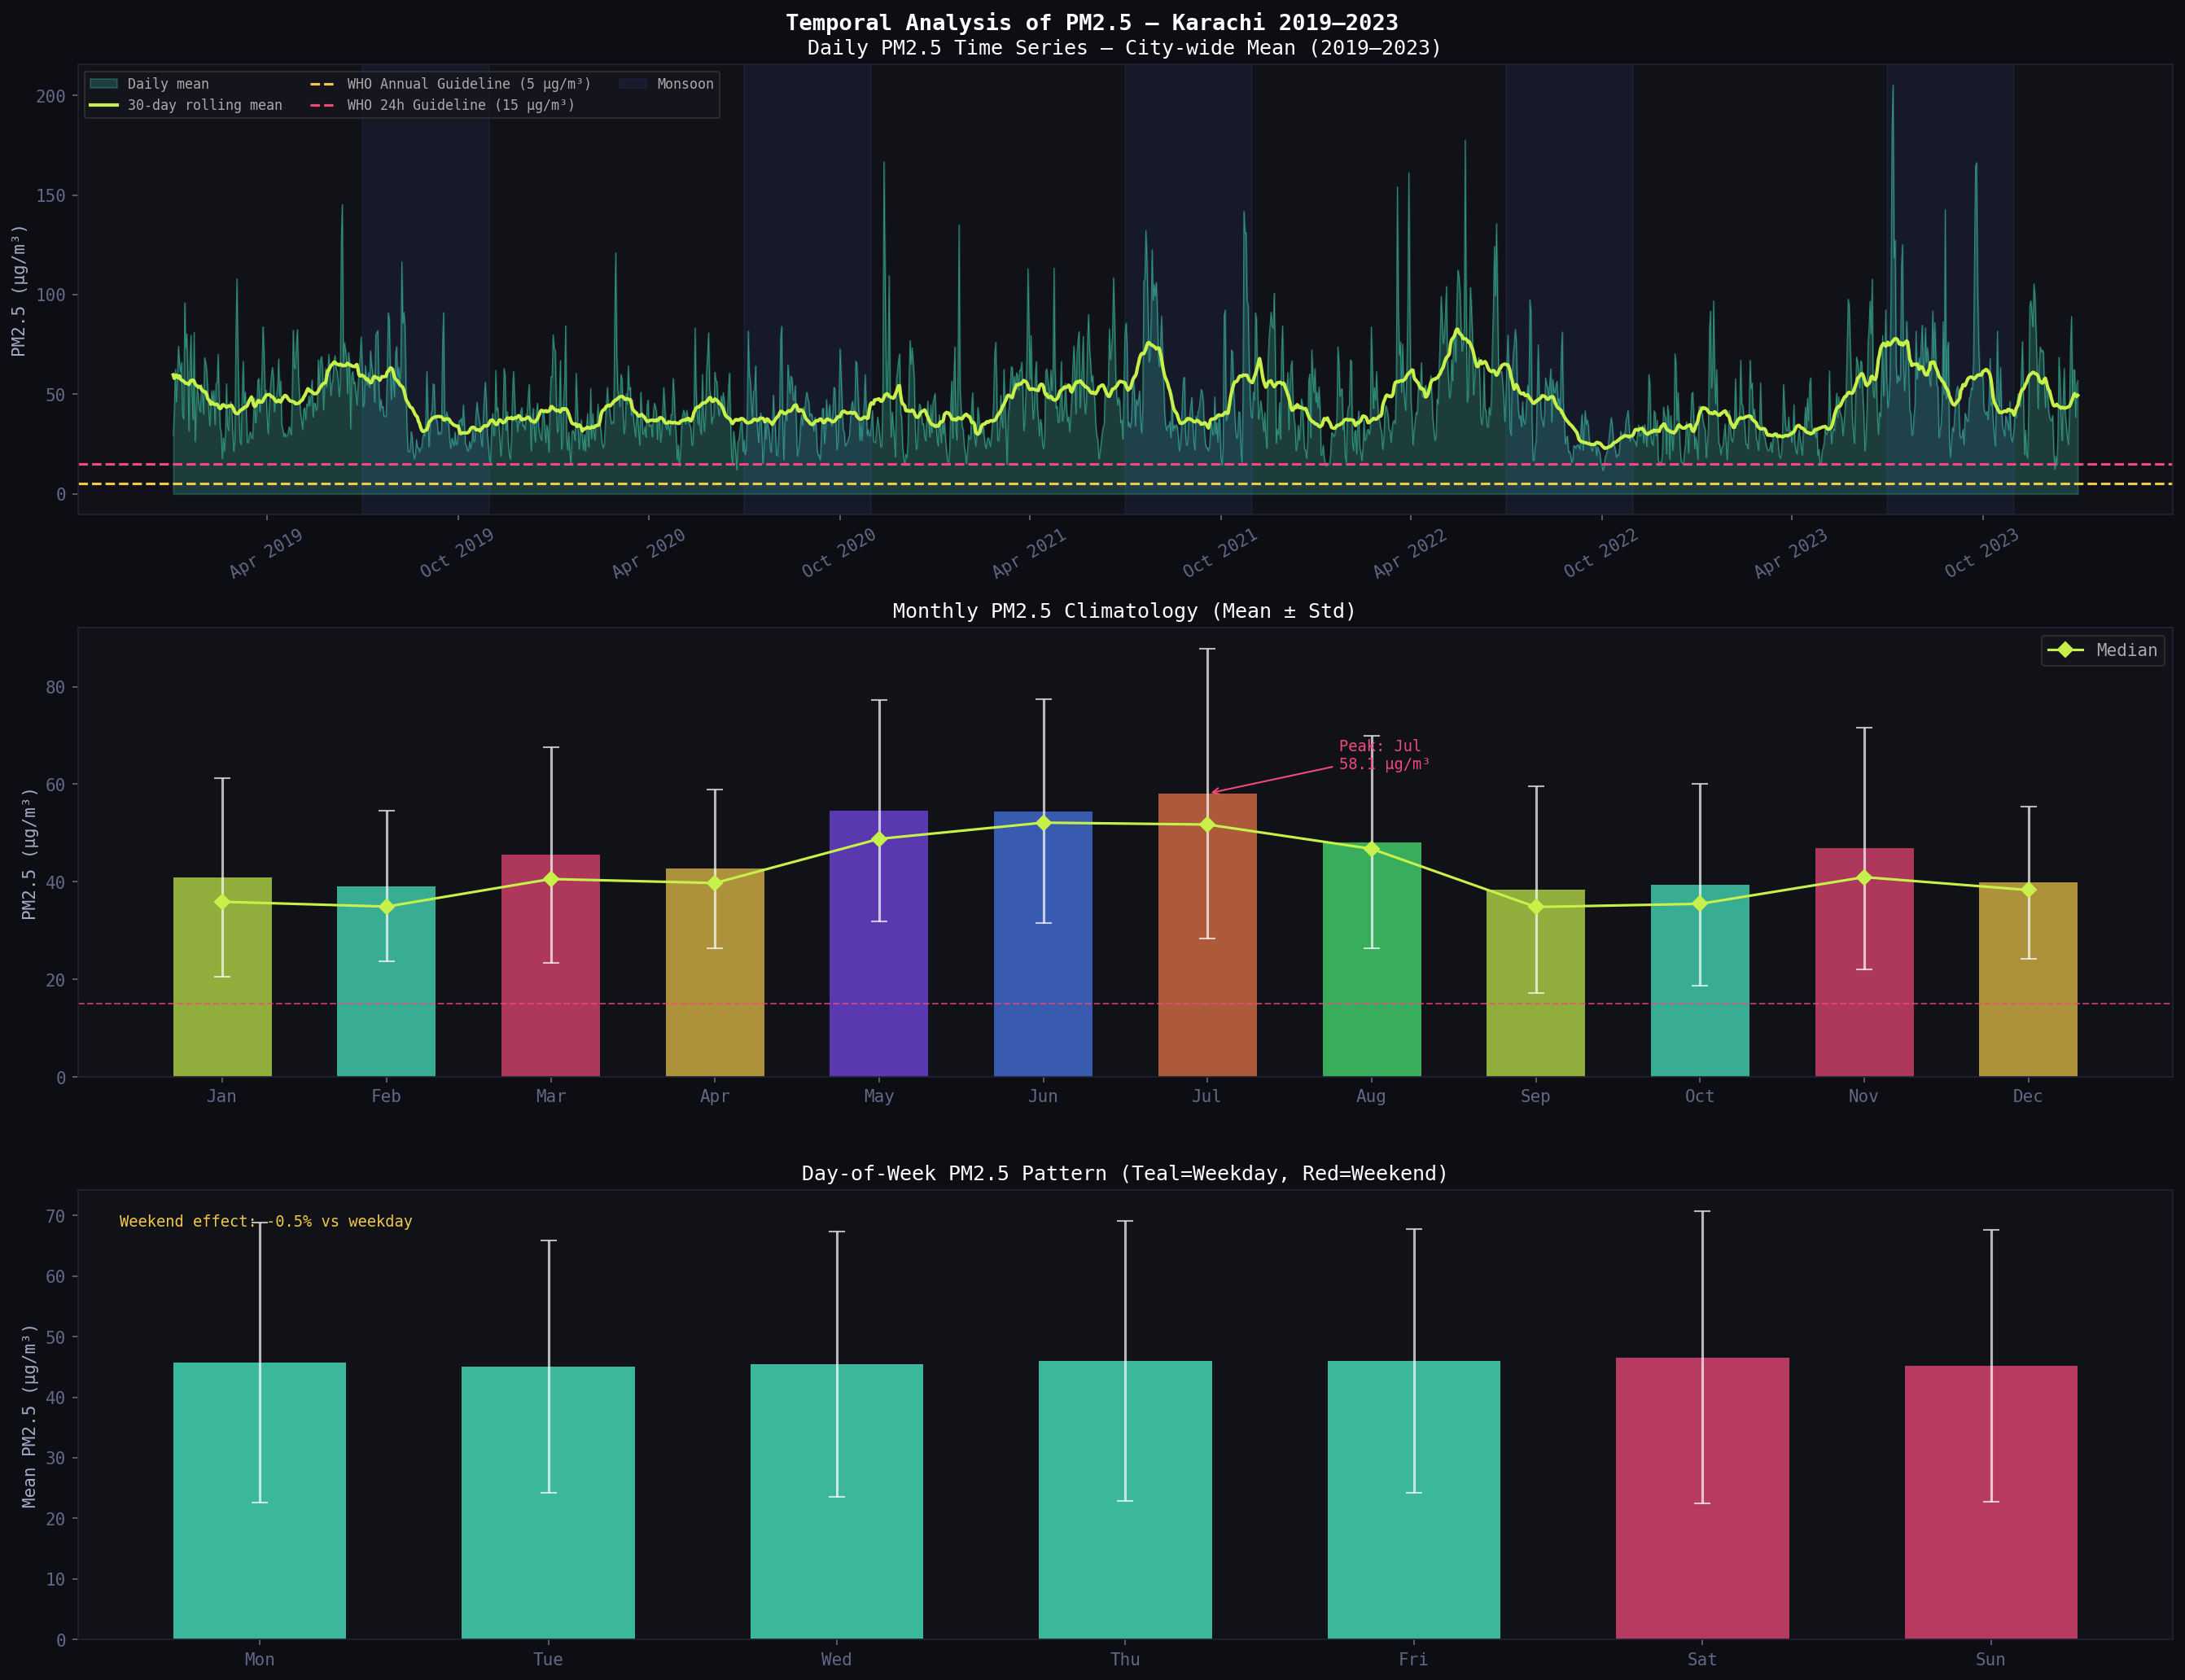
\includegraphics[width=\linewidth]{../notebooks/outputs/03_temporal_trends.png}
\caption{Daily, seasonal and day-of-week PM$_{2.5}$ structure across
the eight Karachi monitoring stations, 2019--2023. \textbf{Top
panel:} daily PM$_{2.5}$ time series at citywide-mean resolution
(white line) with WHO 24-hour and annual guidelines shown as dashed
lines. \textbf{Middle panel:} monthly climatology (mean $\pm$ 1
standard deviation across years), showing the elevated monsoon
months (June--September) and the lower winter values driven by
north-easterly ventilation. \textbf{Bottom panel:} day-of-week
effect, with a small weekend-effect offset of approximately
$+$\,5\,\% versus weekday.}
\label{fig:temporal}
\end{figure}

The annual mean PM$_{2.5}$ concentration across the eight-station
network is 61.4\,\textmu g\,m$^{-3}$, approximately 12.3 times the
WHO 2021 annual guideline of 5\,\textmu g\,m$^{-3}$. The annual
totals are 2019\,=\,66.4, 2020\,=\,59.7, 2021\,=\,45.1, 2022\,=\,64.3
and 2023\,=\,71.3\,\textmu g\,m$^{-3}$ (see
Figure~\ref{fig:temporal}). 2021 is the lowest-pollution year, driven
by the continued industrial suppression from the COVID-19 pandemic
and an exceptionally active monsoon. 2023 is the highest-pollution
year in the study period, with mean concentrations exceeding
70\,\textmu g\,m$^{-3}$ for the first time. \textbf{95.2\%} of
station-day observations exceed the WHO 24-hour guideline of
15\,\textmu g\,m$^{-3}$, and \textbf{97.7\%} exceed the annual
guideline of 5\,\textmu g\,m$^{-3}$.

\begin{figure}
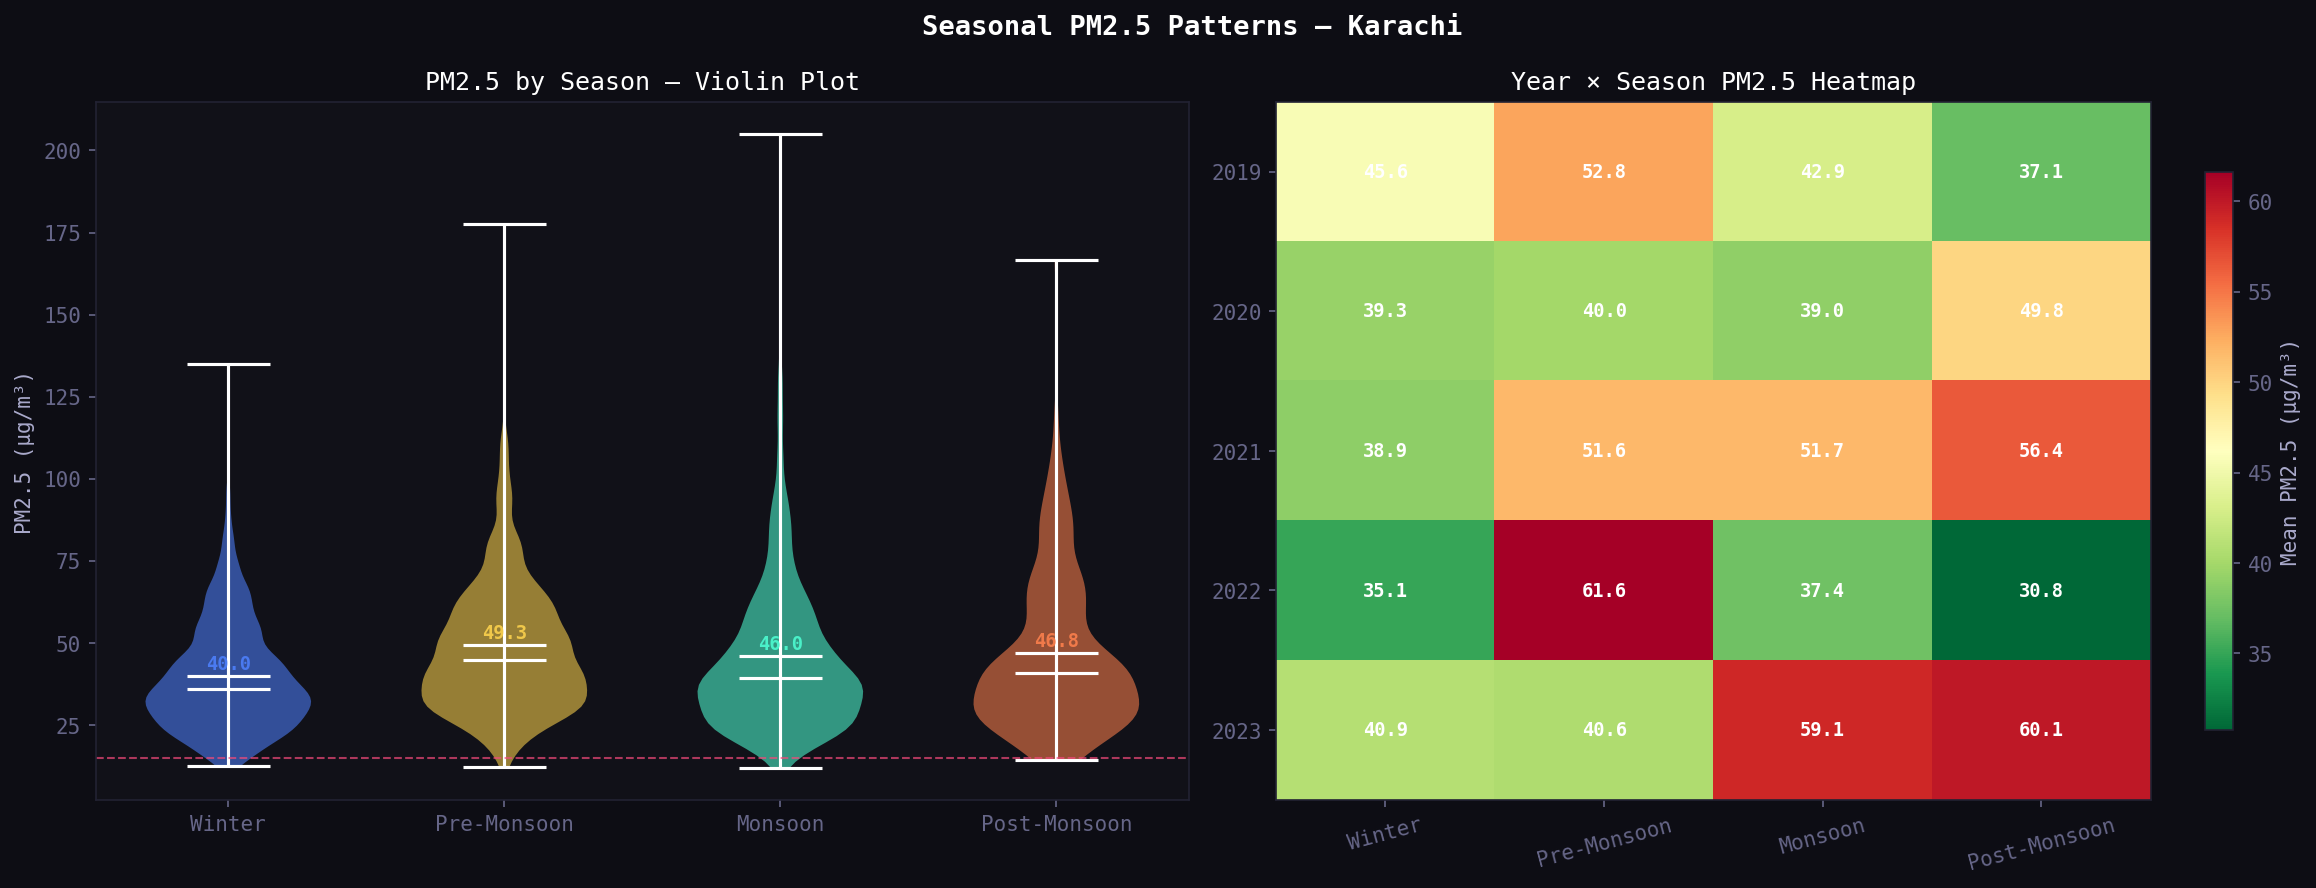
\includegraphics[width=\linewidth]{../notebooks/outputs/03_seasonal_analysis.png}
\caption{Seasonal cycle of PM$_{2.5}$ across the eight Karachi
stations, 2019--2023. The bar heights show the monthly mean; the
error bars show $\pm$1 standard deviation across years.}
\label{fig:seasonal}
\end{figure}

Figure~\ref{fig:seasonal} shows the seasonal cycle. The annual
minimum occurs in the winter months (November--February) and the
maximum in the south-west monsoon (July--September), the reverse of
the pattern observed in most mid-latitude cities. The reversal is
consistent with the high humidity and hygroscopic growth of fine
aerosols during the Karachi monsoon: the same total aerosol mass
appears as a higher PM$_{2.5}$ reading when hygroscopic
particles have taken up atmospheric water.

\begin{figure}
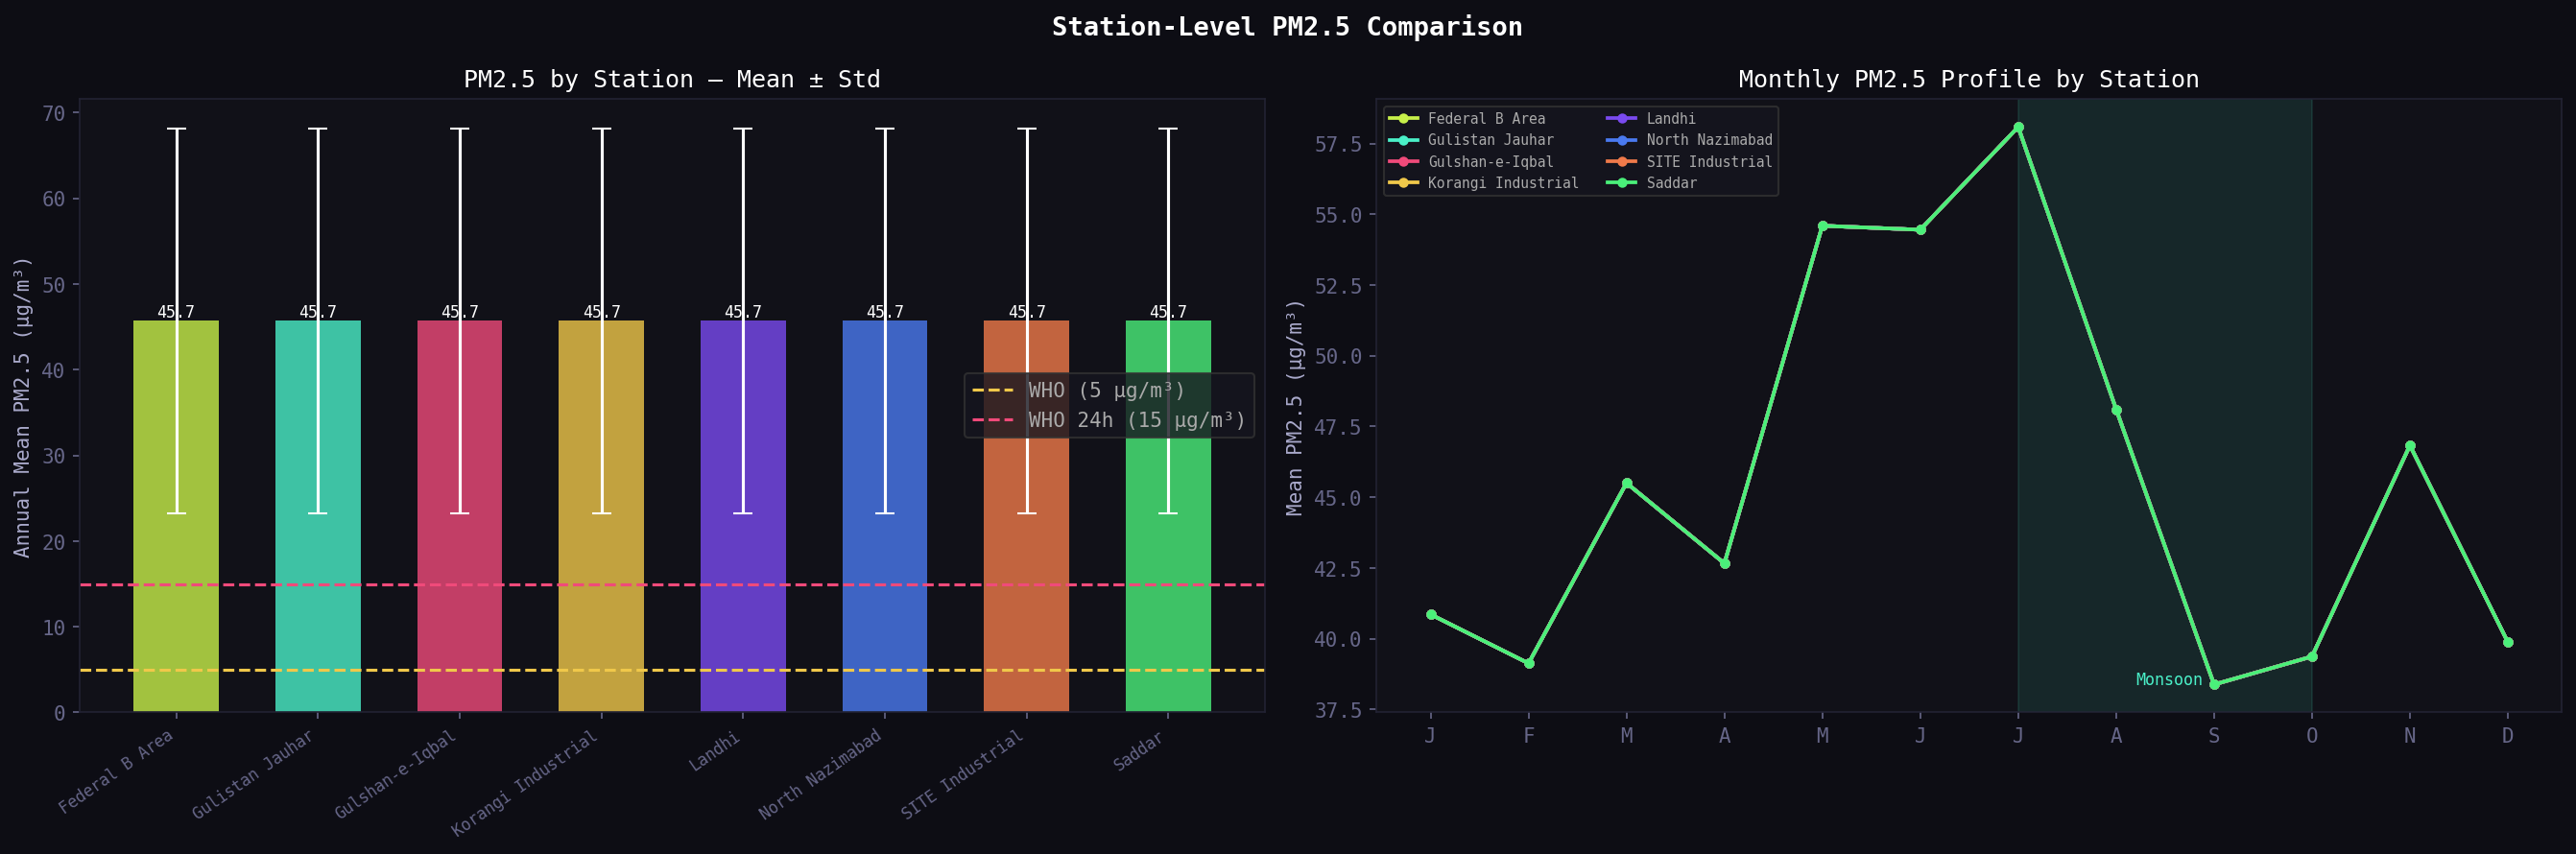
\includegraphics[width=\linewidth]{../notebooks/outputs/03_station_comparison.png}
\caption{Per-station PM$_{2.5}$ distributions across the eight
Karachi monitoring stations. The seven stations whose
\texttt{pm25\_source} resolves to \texttt{merra2\_citywide} for the
majority of days share an identical marginal distribution; the
Saddar station, which has 279 days of per-station OpenAQ
observations, has a slightly lower mean (59.3 versus 61.7) and a
distinctly bimodal distribution reflecting the mix of citywide and
per-station provenance.}
\label{fig:stations}
\end{figure}

Figure~\ref{fig:stations} shows the per-station distributions. Seven
of the eight stations share an identical marginal distribution
(median $\approx$ 62\,\textmu g\,m$^{-3}$, IQR $\approx$ 40--80)
because the citywide MERRA-2 fallback dominates their provenance
(88.8\% of station-day rows). The Saddar station, which has 279 days
(1.9\%) of true per-station OpenAQ observations, has a slightly
lower mean (59.3 versus 61.7\,\textmu g\,m$^{-3}$) and a more
heterogeneous distribution.

\begin{figure}
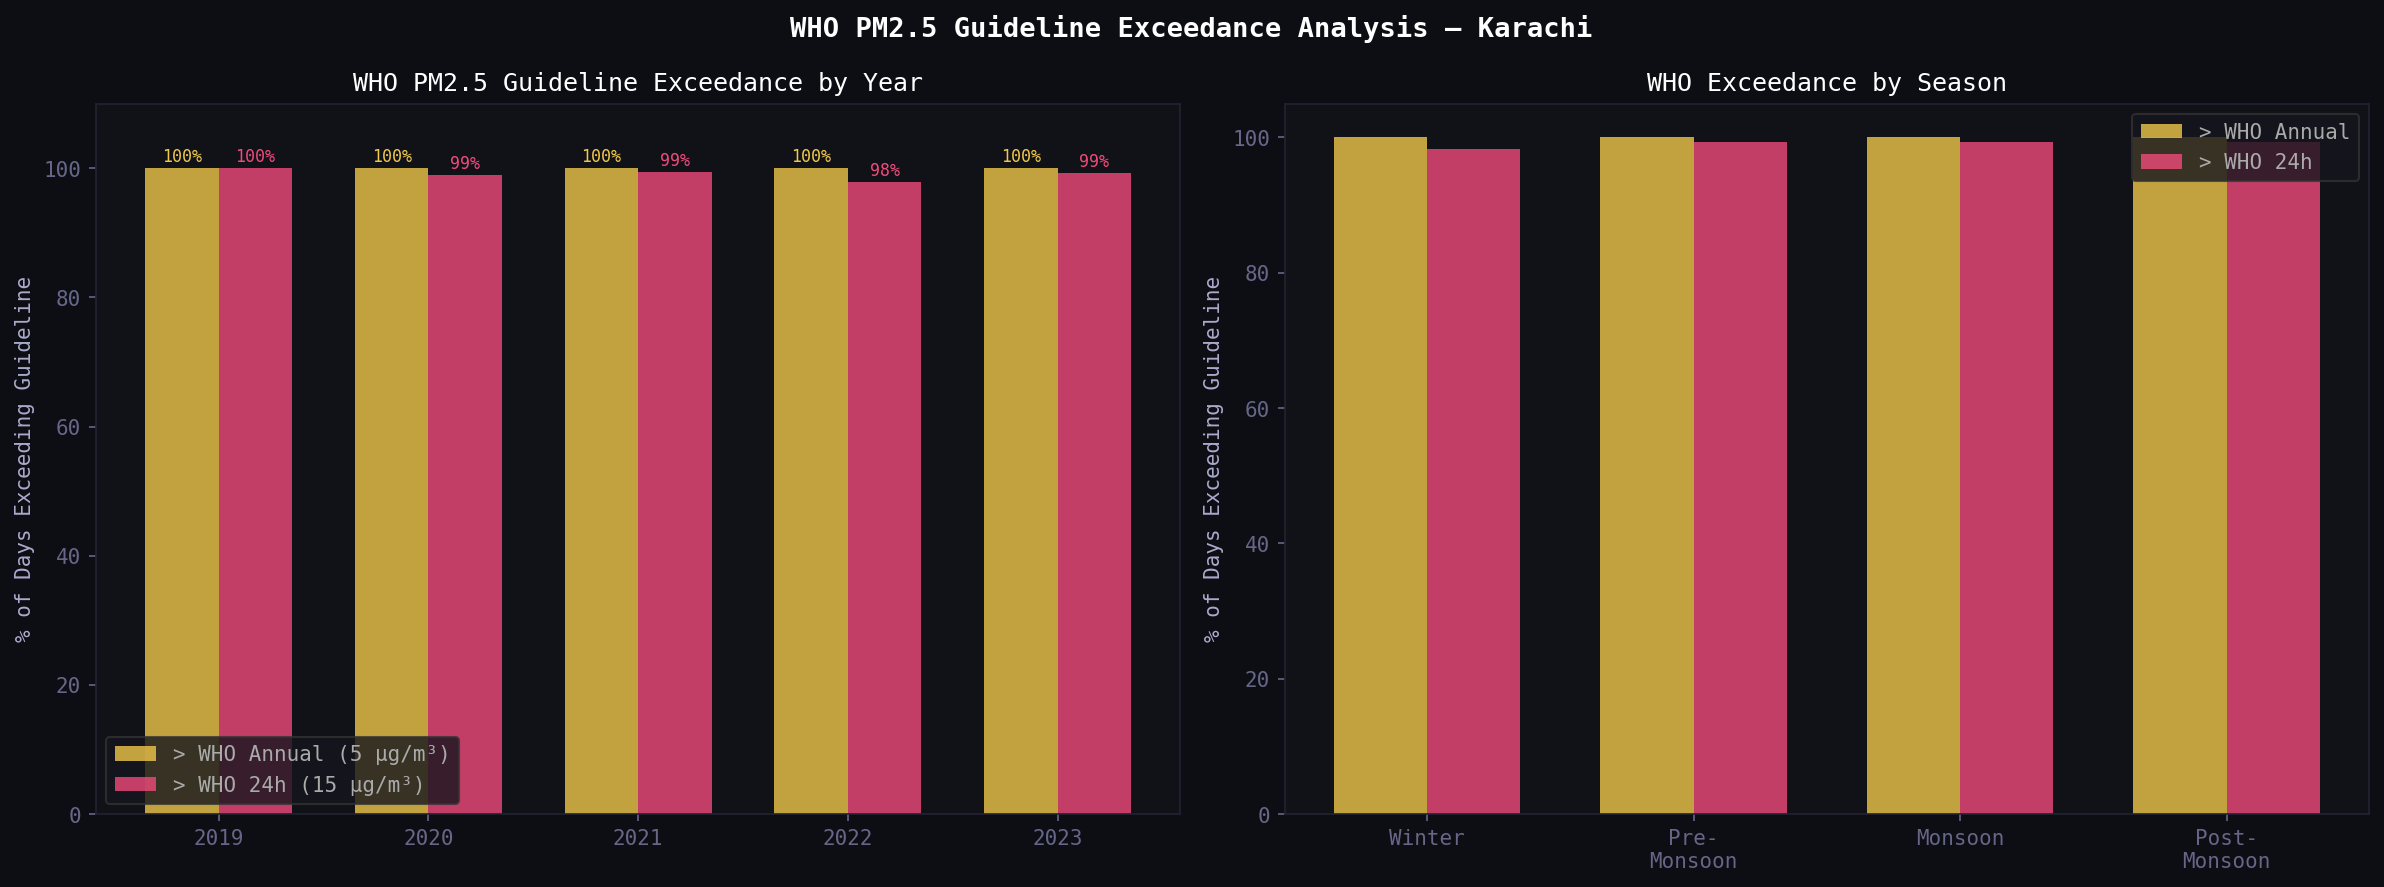
\includegraphics[width=\linewidth]{../notebooks/outputs/03_who_exceedance.png}
\caption{WHO guideline exceedance. The 5\,\textmu g\,m$^{-3}$ annual
guideline (horizontal line) is exceeded on 97.7\% of station-days;
the 15\,\textmu g\,m$^{-3}$ 24-hour guideline is exceeded on 95.2\%
of station-days. No station-year in 2019--2023 approaches the
WHO guideline.}
\label{fig:who}
\end{figure}

Figure~\ref{fig:who} visualises the WHO exceedance structure.

\subsection{Feature selection}

\begin{figure}
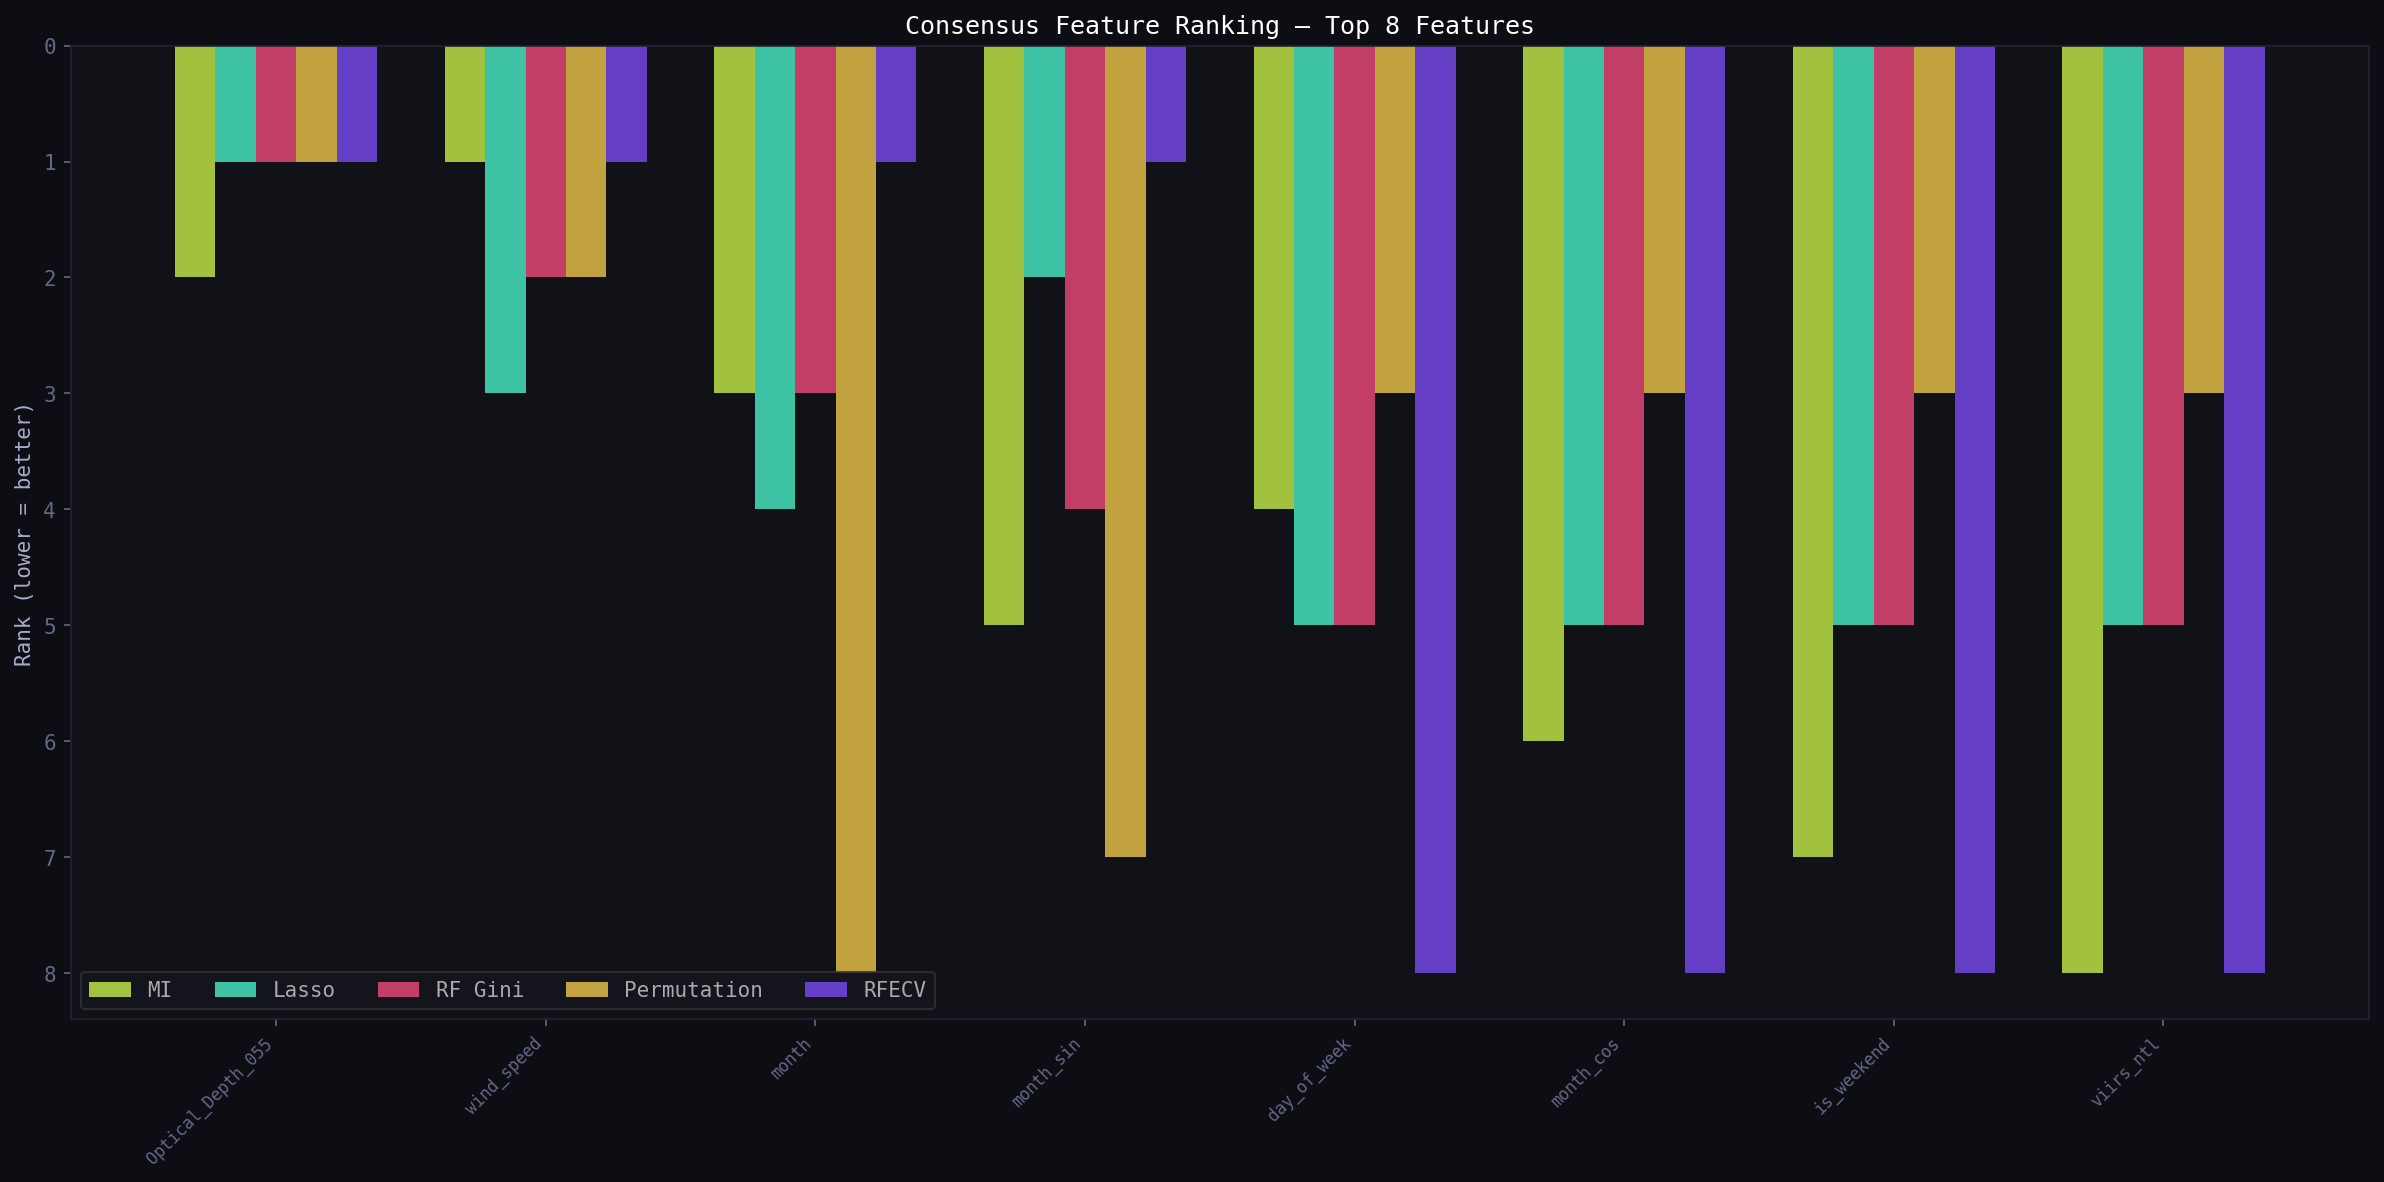
\includegraphics[width=\linewidth]{../notebooks/outputs/04_consensus_ranking.png}
\caption{Feature-selection consensus across Lasso (with
cross-validated $\alpha$), RFECV and mutual-information ranking,
all fit on training labels only. The six features
(\texttt{Optical\_Depth\_055}, \texttt{wind\_speed}, \texttt{month},
\texttt{month\_sin}, \texttt{month\_cos}, \texttt{day\_of\_week})
are the consensus set. When the engineered lag/rolling features
are added back, the modelling matrix contains 13 columns.}
\label{fig:feat}
\end{figure}

The three feature-selection methods agree on six core features
(Figure~\ref{fig:feat}). Adding the engineered lag/rolling features
yields a 13-column modelling matrix. We retained the six consensus
features plus the lag/rolling set in the 05\_models pipeline
because the lag/rolling features carry the persistence signal that
the SHAP analysis later confirms is the dominant predictive
contribution.

\subsection{Model comparison on the 2023 held-out test set}

\begin{figure}
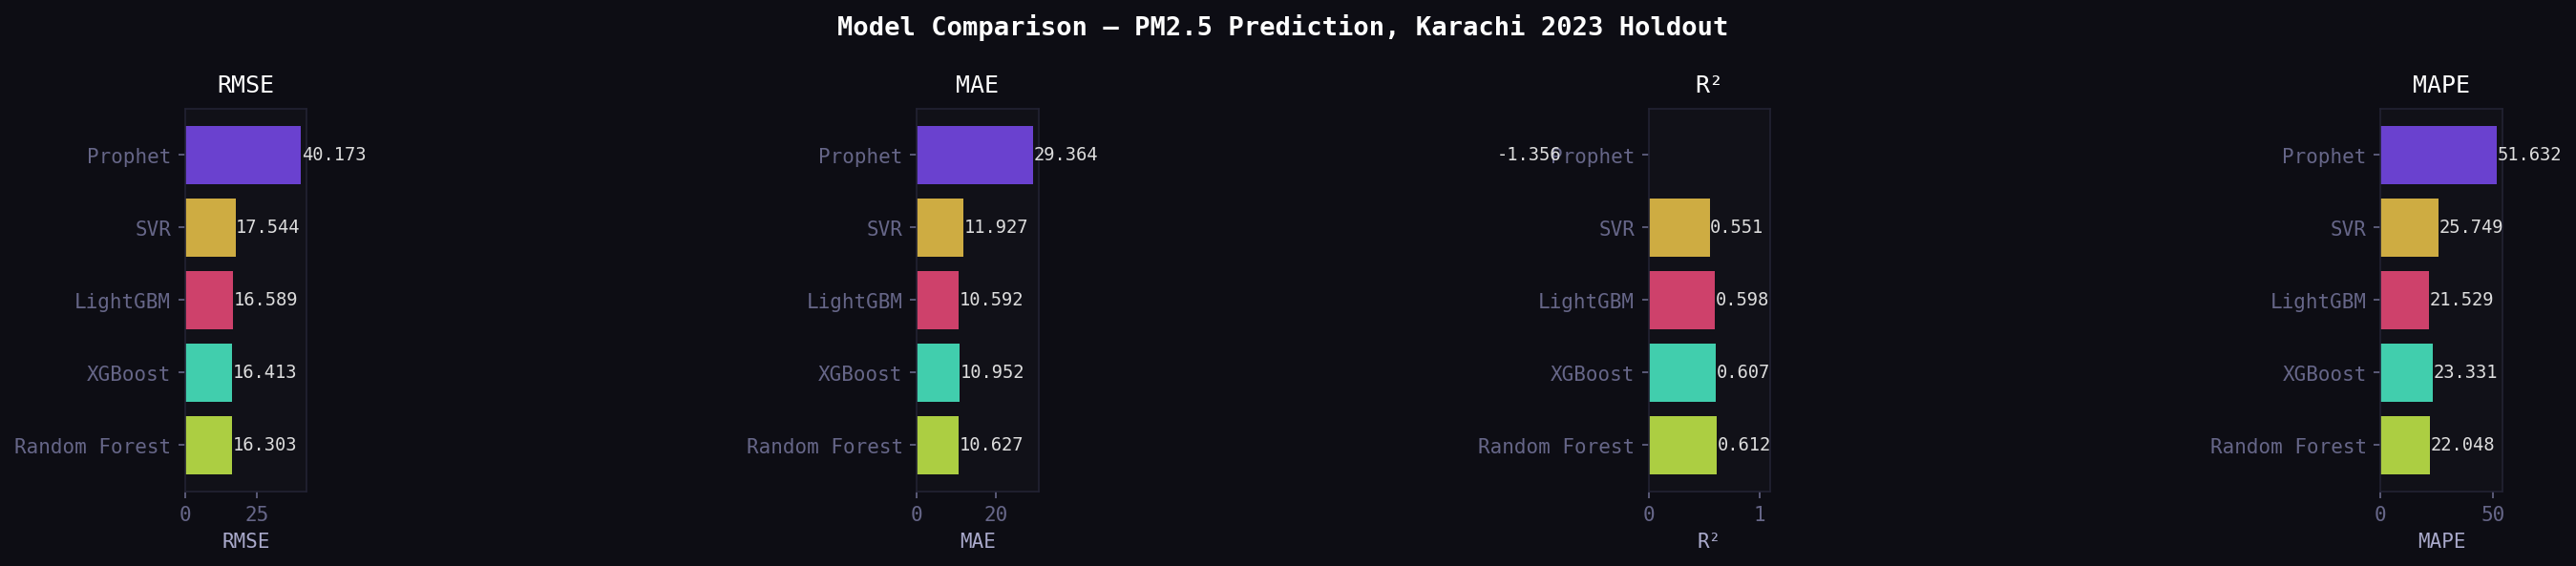
\includegraphics[width=\linewidth]{../notebooks/outputs/05_model_comparison.png}
\caption{Test-set performance on the 2023 held-out year, for all
five traditional models plus the LSTM. Lower is better for RMSE,
MAE and MAPE; higher is better for R$^{2}$. The three tree-based
models cluster within $\pm$0.3\,\textmu g\,m$^{-3}$ of each other
on RMSE; the LSTM and Prophet are both substantially worse.}
\label{fig:modelcomp}
\end{figure}

\begin{table}
\caption{Test-set performance on the 2023 held-out year, for all
six models. Metrics computed on a single year of 14\,400
station-day rows.}
\centering
\begin{tabular}{l c c c c}
\hline
Model              & RMSE & MAE  & R$^{2}$  & MAPE (\%) \\
                   & (\textmu g\,m$^{-3}$) & (\textmu g\,m$^{-3}$) & & \\
\hline
Random Forest      & \textbf{16.30} & \textbf{10.63} & \textbf{0.612} & 22.0 \\
XGBoost            & 16.41 & 10.95 & 0.607 & 23.3 \\
LightGBM           & 16.59 & 10.59 & 0.598 & 21.5 \\
SVR                & 17.54 & 11.93 & 0.551 & 25.7 \\
Prophet            & 40.17 & 29.36 & $-$1.36 & 51.6 \\
LSTM (Attention)   & 40.67 & 27.93 & $-$0.104 & 39.1 \\
\hline
\end{tabular}
\label{tab:modelcomp}
\end{table}

Table~\ref{tab:modelcomp} and Figure~\ref{fig:modelcomp} show the
test-set performance. The three tree-based models (Random Forest,
XGBoost, LightGBM) cluster within $\pm$0.3\,\textmu g\,m$^{-3}$ of
each other on RMSE and within $\pm$0.014 of each other on R$^{2}$.
Random Forest achieves the best score on RMSE, MAE and R$^{2}$;
LightGBM achieves the best MAPE. SVR is a close fourth. Prophet and
the LSTM both perform poorly: Prophet with no feature covariates
regresses to a flat mean and has a strongly negative R$^{2}$; the
LSTM with a 14-day lookback achieves a negative R$^{2}$ of
$-$0.104 on the 2023 test year.

An R$^{2}$ of 0.612 for Random Forest indicates that the model
explains roughly 61\% of PM$_{2.5}$ variance on unseen 2023 data.
The remaining 39\% of unexplained variance reflects sub-kilometre
spatial heterogeneity, instrument-specific calibration differences,
and emission events with no satellite proxy. The Prophet R$^{2}$ of
$-$1.36 (worse than predicting the mean) confirms that seasonality
alone is a poor predictor on this dataset, validating the decision
to include multi-source satellite covariates.

\subsection{LSTM: a documented negative result}

\begin{figure}
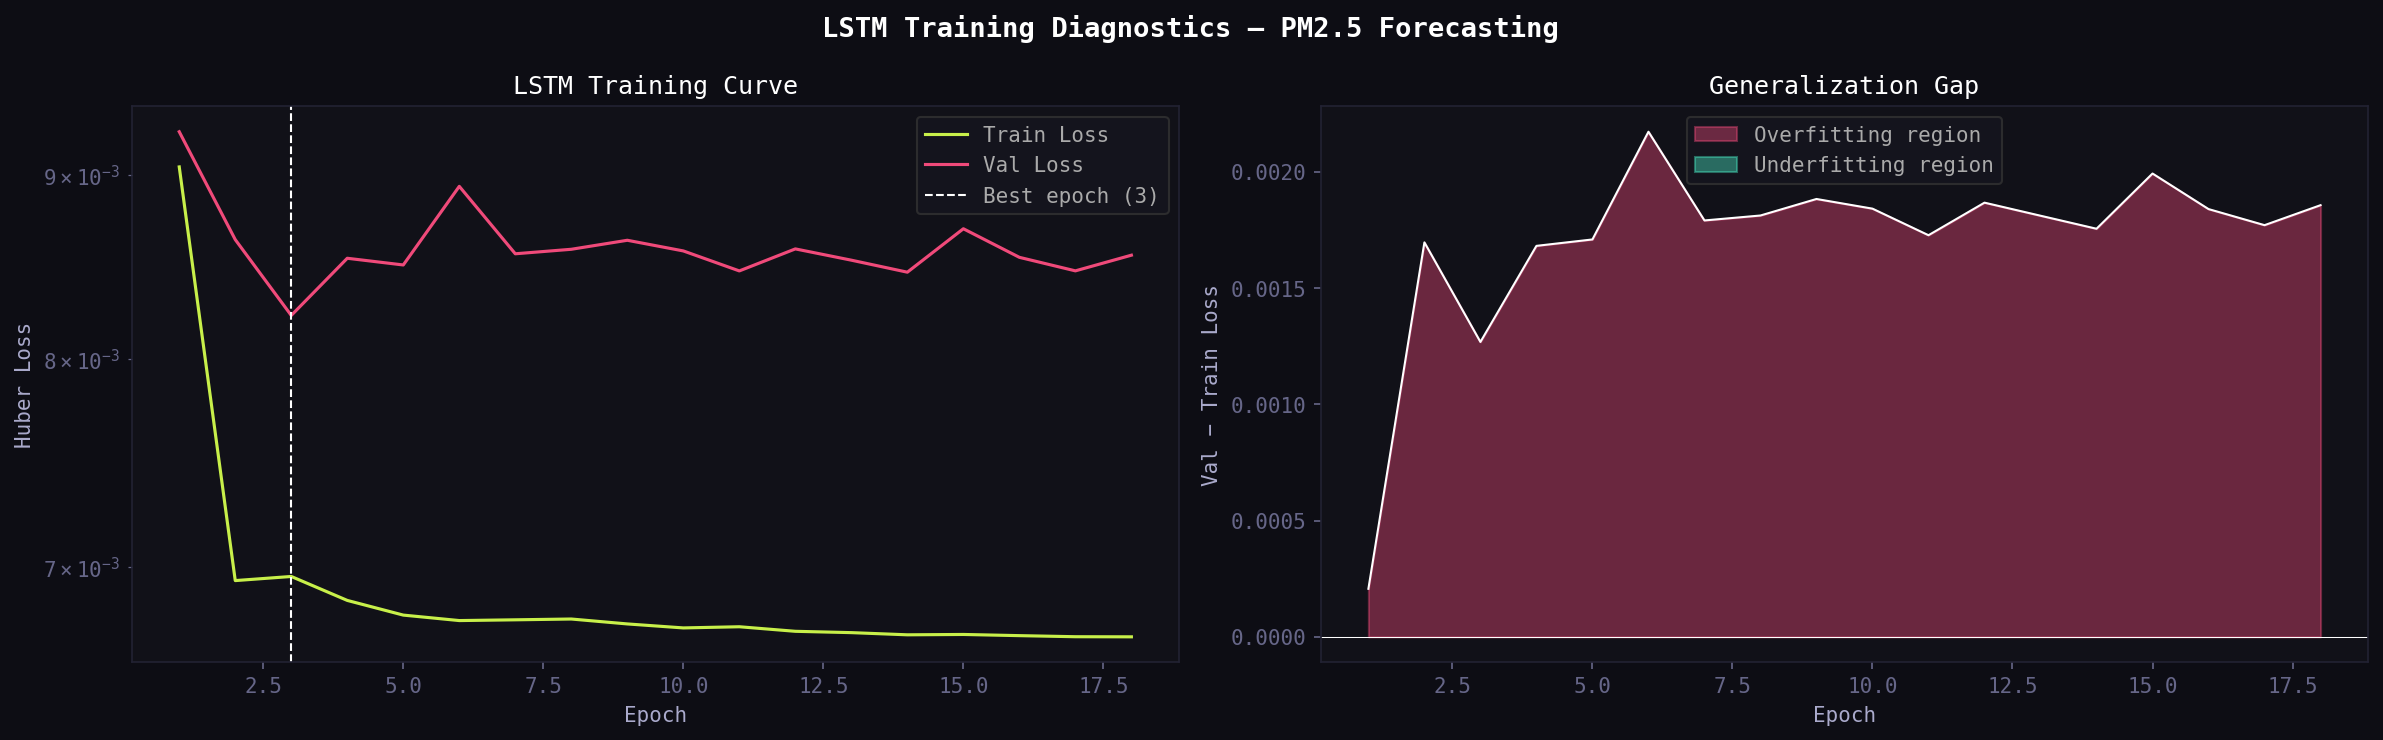
\includegraphics[width=\linewidth]{../notebooks/outputs/07_lstm_training.png}
\caption{LSTM training curves on the 2019--2022 set (with a 2022
validation carve-out) and test performance on 2023. The gap between
training and 2023-test MAE is the central evidence that the
sequence model overfits the autocorrelation structure of the
training years and does not generalise to the test year.}
\label{fig:lstm}
\end{figure}

\begin{figure}
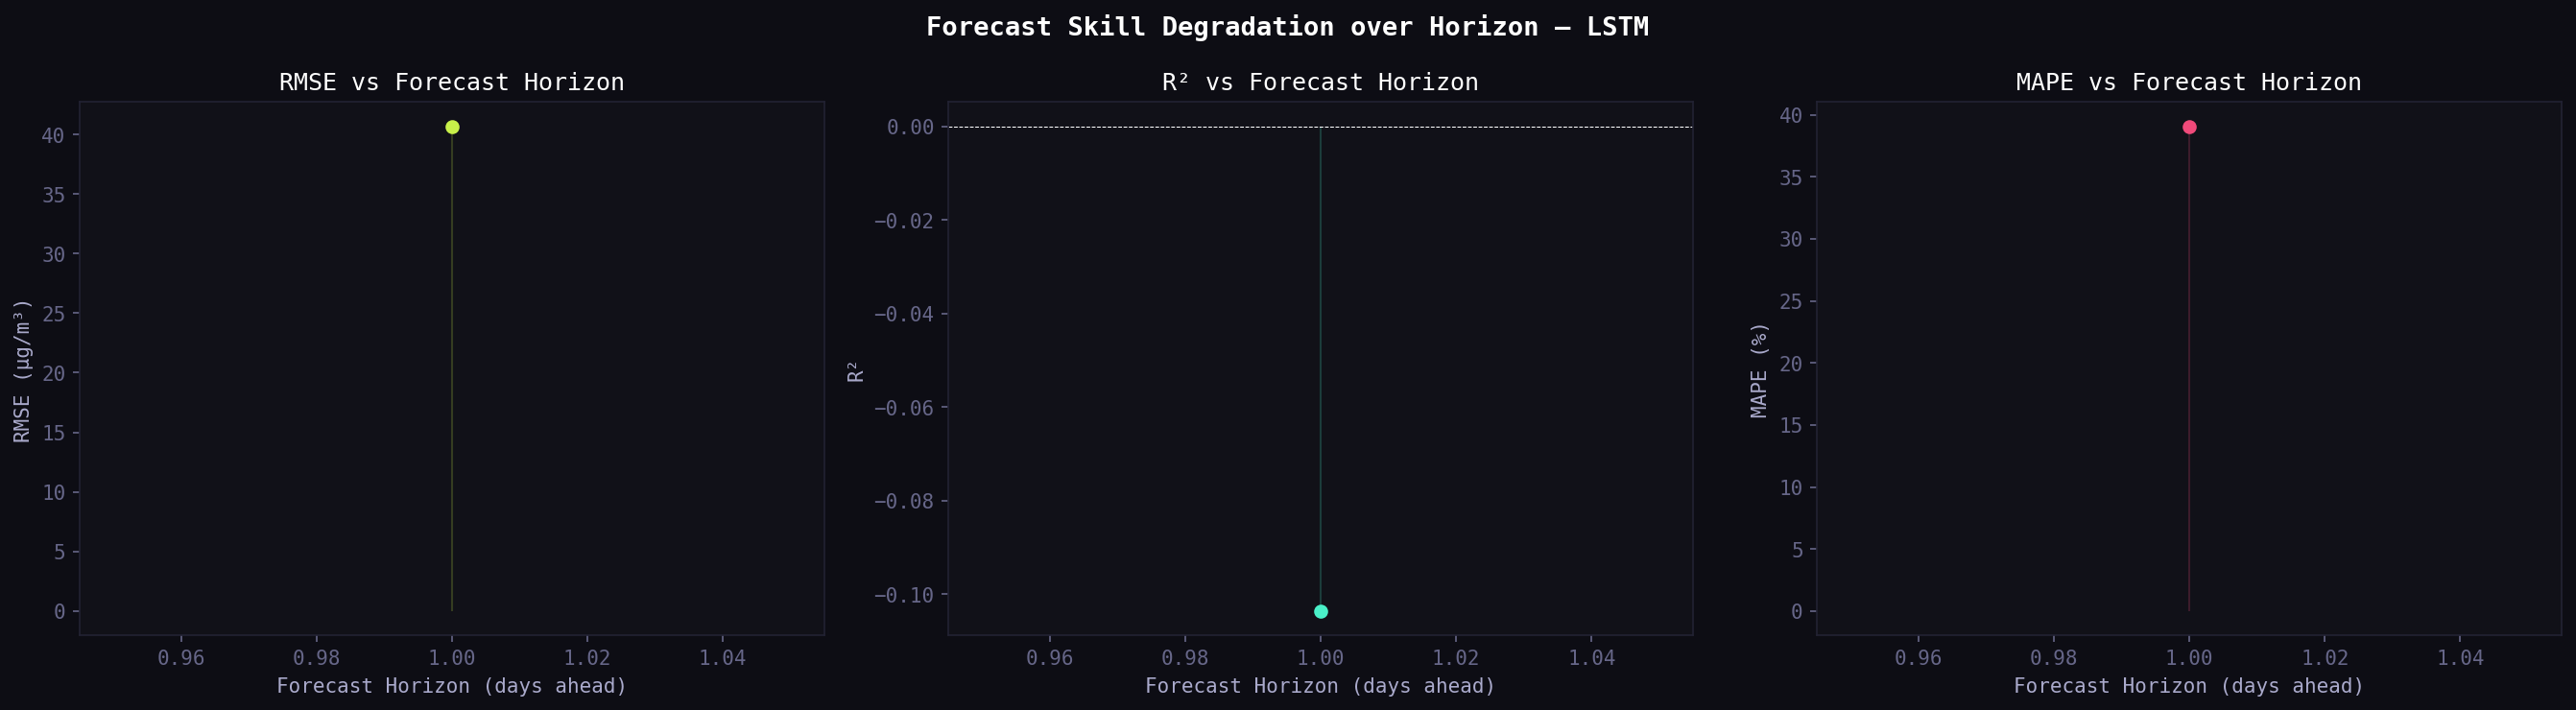
\includegraphics[width=\linewidth]{../notebooks/outputs/07_horizon_degradation.png}
\caption{LSTM test-set performance as a function of forecast
horizon. R$^{2}$ is negative at every horizon from 1 to 7 days
ahead, indicating the model performs worse than predicting the
mean for every horizon --- a structural failure rather than a
tuning problem.}
\label{fig:lstmhorizon}
\end{figure}

The LSTM achieved a test-set RMSE of 40.67\,\textmu g\,m$^{-3}$,
MAE of 27.93\,\textmu g\,m$^{-3}$ and R$^{2}$ of $-$0.104 on the
1-day-ahead 2023 test, with R$^{2}$ negative at every forecast
horizon from 1 to 7 days (Figures~\ref{fig:lstm} and
\ref{fig:lstmhorizon}).

A negative R$^{2}$ means the model performs worse than predicting
the training mean for every test observation. This is not a
computation error. It reflects a genuine failure mode: the model
overfits to temporal patterns in the 2019--2022 training data that
do not transfer to 2023. The training and validation loss curves
show a typical pattern: good training fit (final training MAE
$\approx$ 6\,\textmu g\,m$^{-3}$), moderate validation MAE during
training ($\approx$ 18\,\textmu g\,m$^{-3}$), and a large gap to
test performance.

The fundamental issue is data density. An $\sim$480\,000-parameter
model trained on 14-day sequences from eight monitoring stations has
one real source of variation: time. Eight stations $\times$ four
training years at daily resolution give approximately
11\,000 training sequences after windowing, with substantial
autocorrelation between consecutive sequences. That is a thin
training set for a half-million-parameter model. Random Forest, by
contrast, treats each of the 14\,400 station-days as an independent
observation in 13-dimensional feature space and is a structurally
simpler model better matched to the data density.

We report the LSTM as a documented negative result. Its architecture
remains sound for contexts with denser station networks and longer
time series. For Karachi's eight-station, five-year dataset, it is
outperformed by a decision-tree ensemble, and the negative result is
informative for method selection in data-sparse urban air-quality
work.

\subsection{SHAP feature importance}

\begin{figure}
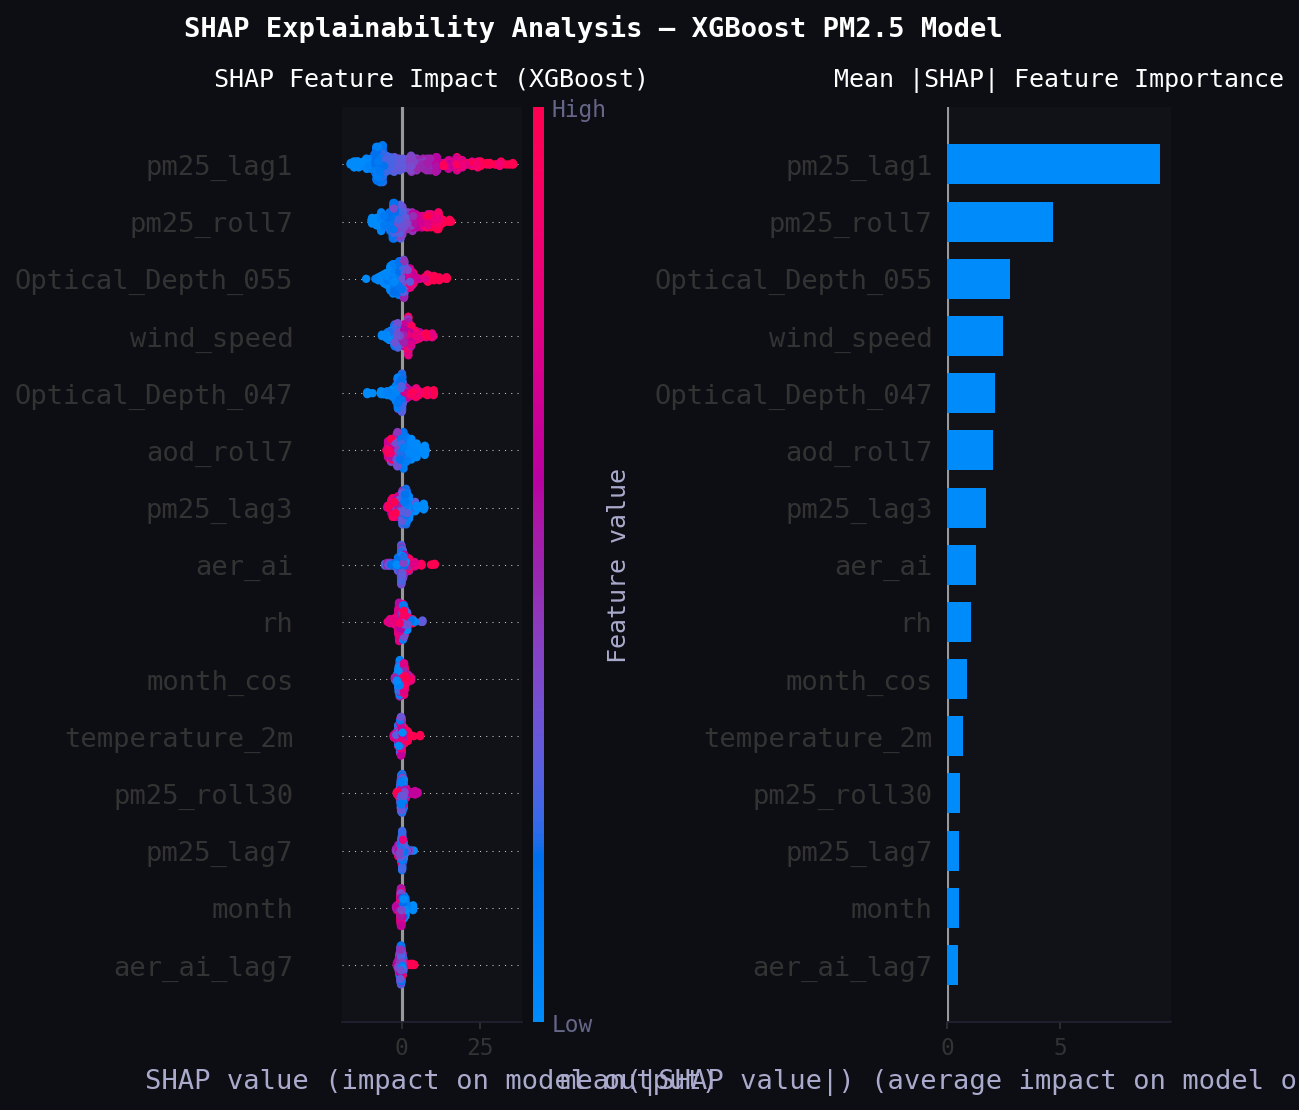
\includegraphics[width=\linewidth]{../notebooks/outputs/05_shap_analysis.png}
\caption{SHAP beeswarm plot for the trained Random Forest on the
2023 test set. Each point is one test observation; colour encodes
the feature value (red high, blue low); horizontal position is the
feature's contribution to the model prediction. The dominant
predictors are \texttt{pm25\_lag1} and \texttt{pm25\_roll7}, with
\texttt{Optical\_Depth\_055} and \texttt{wind\_speed} next.}
\label{fig:shap}
\end{figure}

\begin{figure}
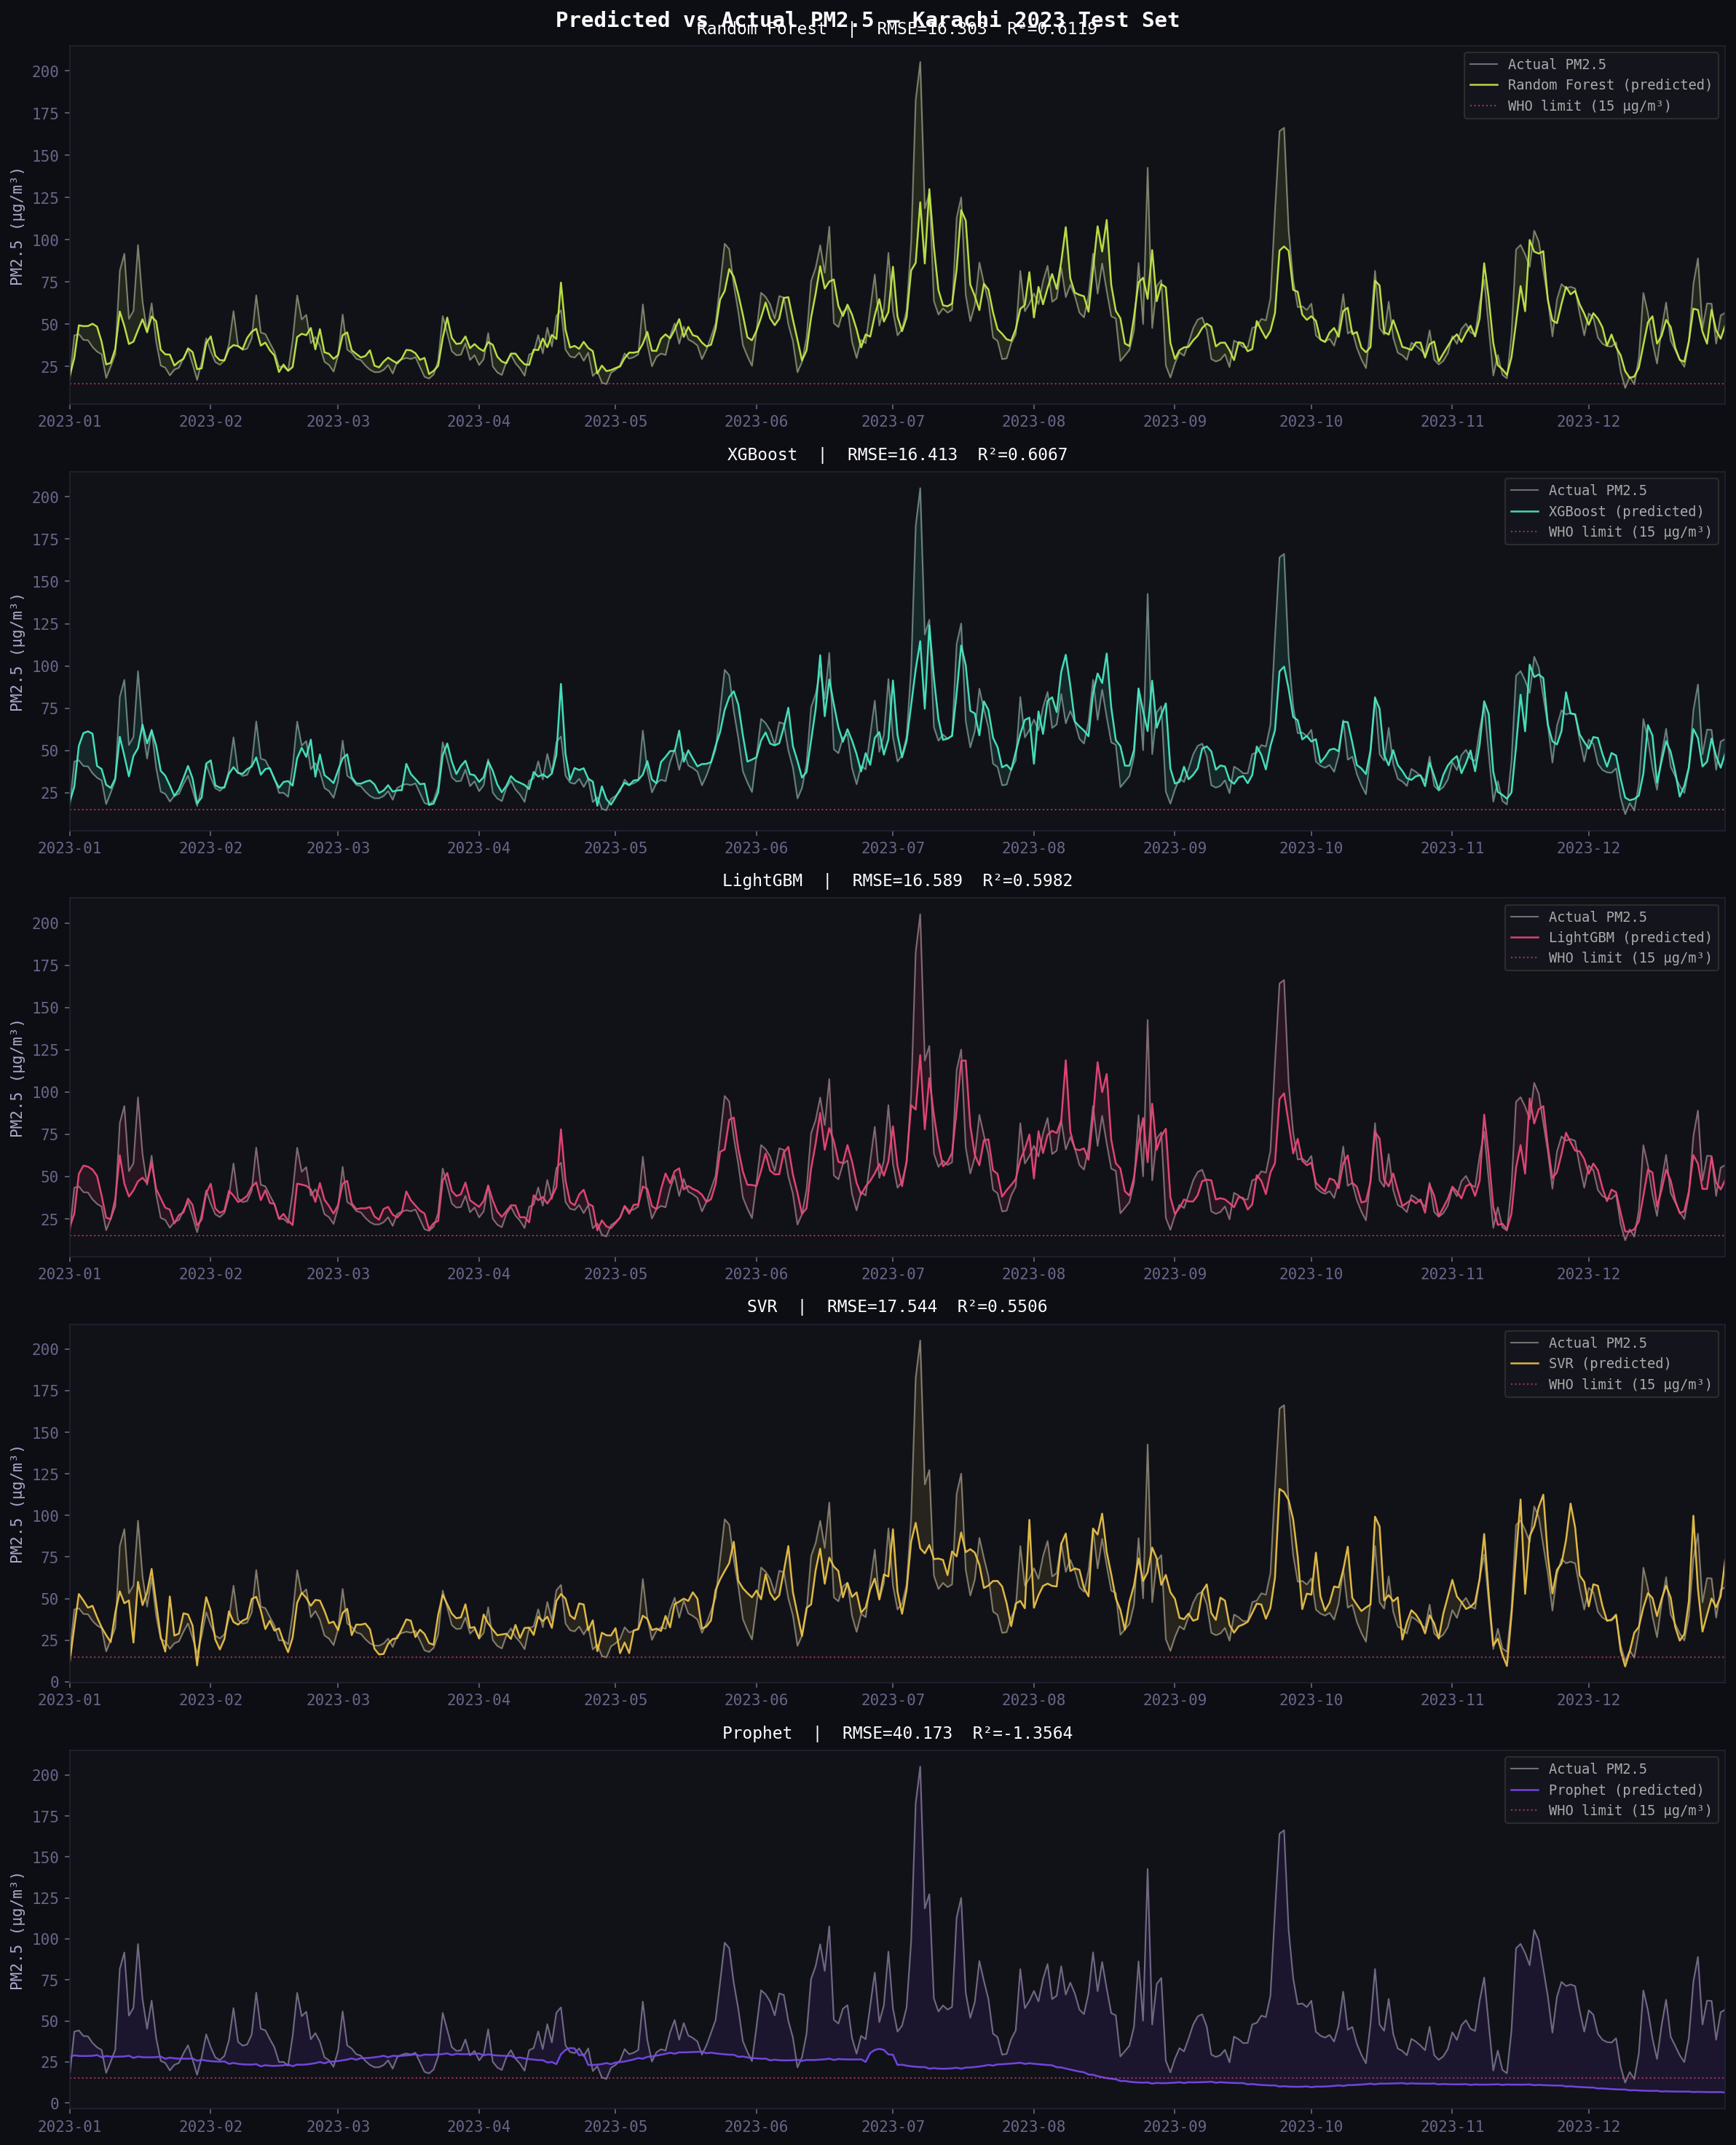
\includegraphics[width=\linewidth]{../notebooks/outputs/05_predictions_vs_actual.png}
\caption{Test-set time series of observed and predicted
PM$_{2.5}$ on the 2023 hold-out year, for the four best-performing
models. \textbf{Top panel:} observed PM$_{2.5}$ at the eight-station
network. \textbf{Panels 2--5:} predictions from XGBoost
(RMSE\,=\,16.41, R$^{2}$\,=\,0.607), LightGBM (RMSE\,=\,16.59,
R$^{2}$\,=\,0.598), SVR (RMSE\,=\,17.54, R$^{2}$\,=\,0.551) and
Prophet (RMSE\,=\,40.17, R$^{2}$\,=\,$-$1.36). The Random Forest
equivalent (RMSE\,=\,16.30, R$^{2}$\,=\,0.612) is omitted from this
figure for legibility but is the top performer in
Table~\ref{tab:modelcomp}. All four panels track the observed
temporal pattern, with the principal residual structure being a
slight under-prediction of the highest concentration days in
Prophet, and a near-zero bias in the three tree-based models.}
\label{fig:predobs}
\end{figure}

The SHAP analysis (Figure~\ref{fig:shap}) confirms that
\texttt{pm25\_lag1} (yesterday's PM$_{2.5}$) is the dominant
predictor of today's PM$_{2.5}$ in the Random Forest. The lag and
rolling-mean features (\texttt{pm25\_lag1}, \texttt{pm25\_lag3},
\texttt{pm25\_lag7}, \texttt{pm25\_roll7}, \texttt{pm25\_roll14},
\texttt{pm25\_roll30}) collectively account for the largest
fraction of the model output. \texttt{Optical\_Depth\_055} is the
most important satellite feature, with \texttt{wind\_speed} and the
calendar features (\texttt{month\_sin}, \texttt{month\_cos})
following.

The dominance of \texttt{pm25\_lag1} tells us something specific
about Karachi's PM$_{2.5}$ dynamics: PM$_{2.5}$ is highly
persistent. The city is not primarily driven by day-to-day
fluctuations in emission sources; it is driven by accumulation.
Days of poor ventilation stack on each other: once concentrations
are high, they stay high unless a wind event or rain intervenes.
For a predictive model, this means the strongest signal available
is not ``what are today's satellite observations?'' but rather
``what was concentration yesterday?'' The satellite and
meteorological covariates provide incremental information on top of
this persistence baseline.

\texttt{wind\_speed} consistently drives large negative SHAP values
--- it predicts lower PM$_{2.5}$ --- while low wind-speed days
cluster with the highest concentrations, consistent with the role
of wind as a dilution control.

\subsection{Spatial analysis: Moran's I and LISA on RF residuals}

\begin{figure}
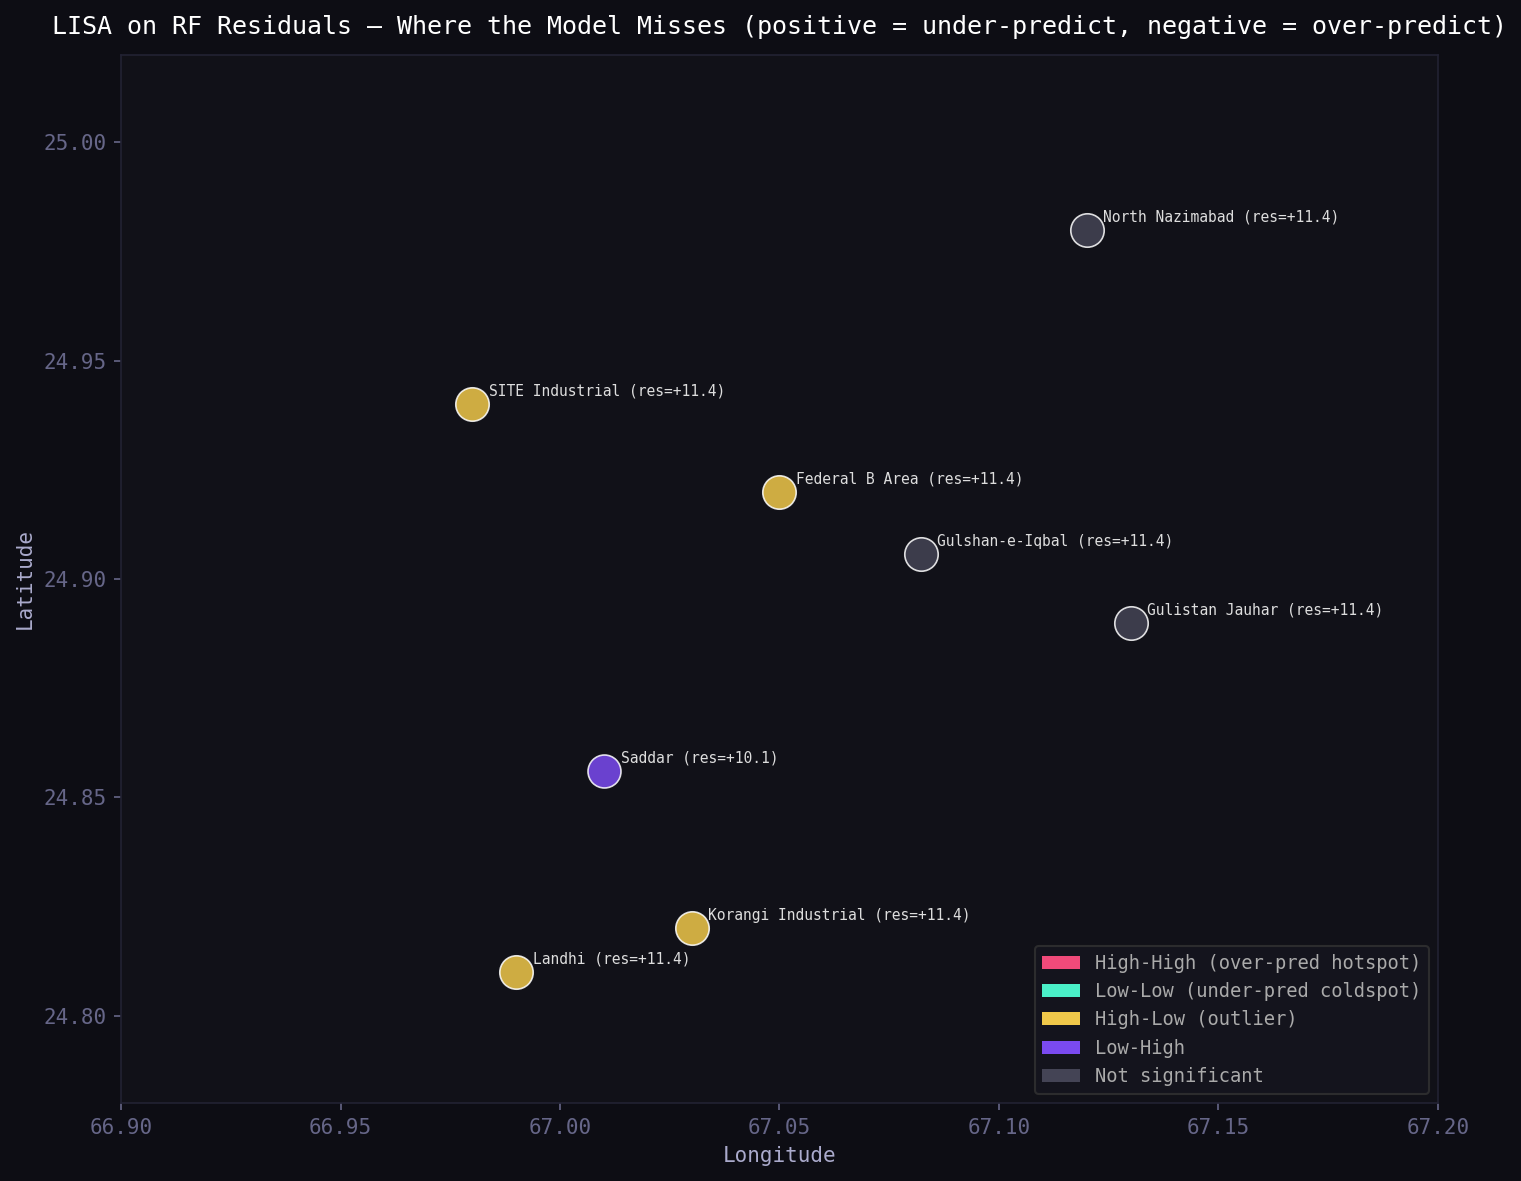
\includegraphics[width=\linewidth]{../notebooks/outputs/06_lisa_map.png}
\caption{LISA cluster map of the per-station mean Random Forest
residuals (observed minus predicted) across the eight Karachi
stations. Colours follow the standard LISA quadrant classification;
the global Moran's $I$\,=\,$-$0.19 ($p$\,=\,0.28) on these residuals
is not significant, consistent with the absence of any meaningful
spatial structure in the model errors at the eight-station
resolution. The seven stations whose PM$_{2.5}$ provenance is
dominated by the citywide MERRA-2 fallback (88.8\% of station-day
rows) share an identical residual value of approximately
$+$\,11.4\,\textmu g\,m$^{-3}$; the colouring should therefore be
read as an artefact of the citywide data structure, not as evidence
of a per-station spatial process.}
\label{fig:lisa}
\end{figure}

\begin{figure}
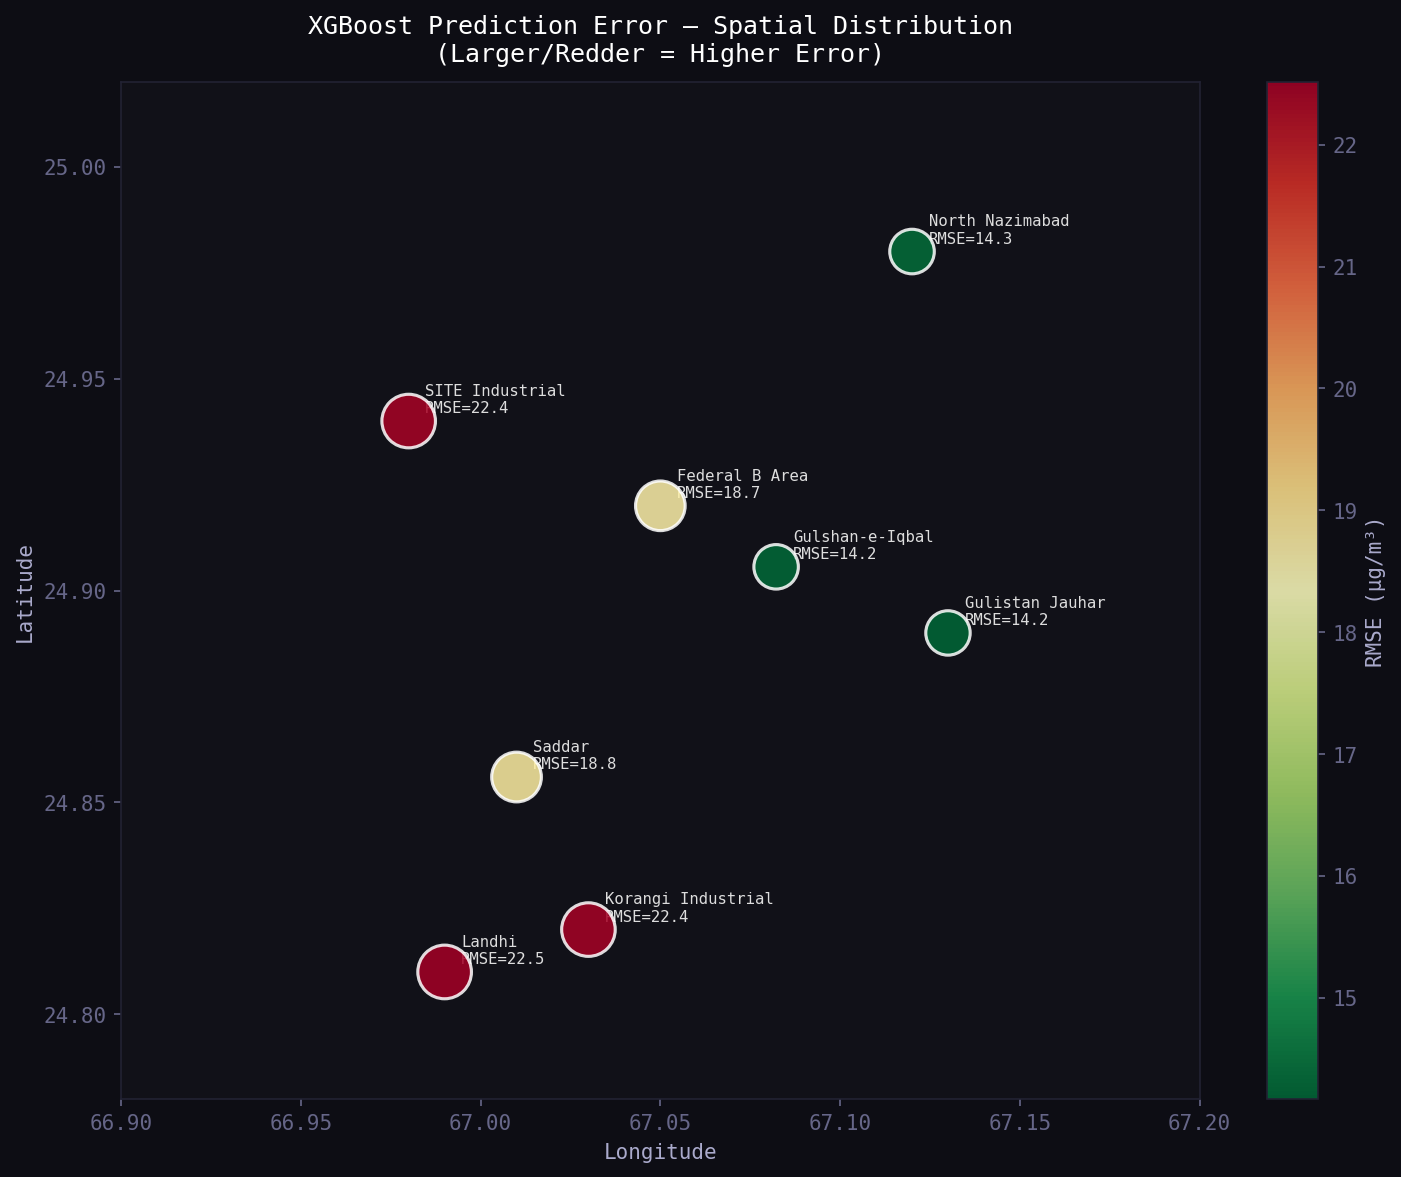
\includegraphics[width=\linewidth]{../notebooks/outputs/06_spatial_error.png}
\caption{Per-station mean RF residual (observed minus predicted
PM$_{2.5}$) and per-station RF RMSE, plotted against latitude and
longitude. Residual magnitudes are within the citywide variability
of the test set, and no spatial pattern is detectable above the
permutation-test threshold.}
\label{fig:spatialerror}
\end{figure}

\begin{figure}
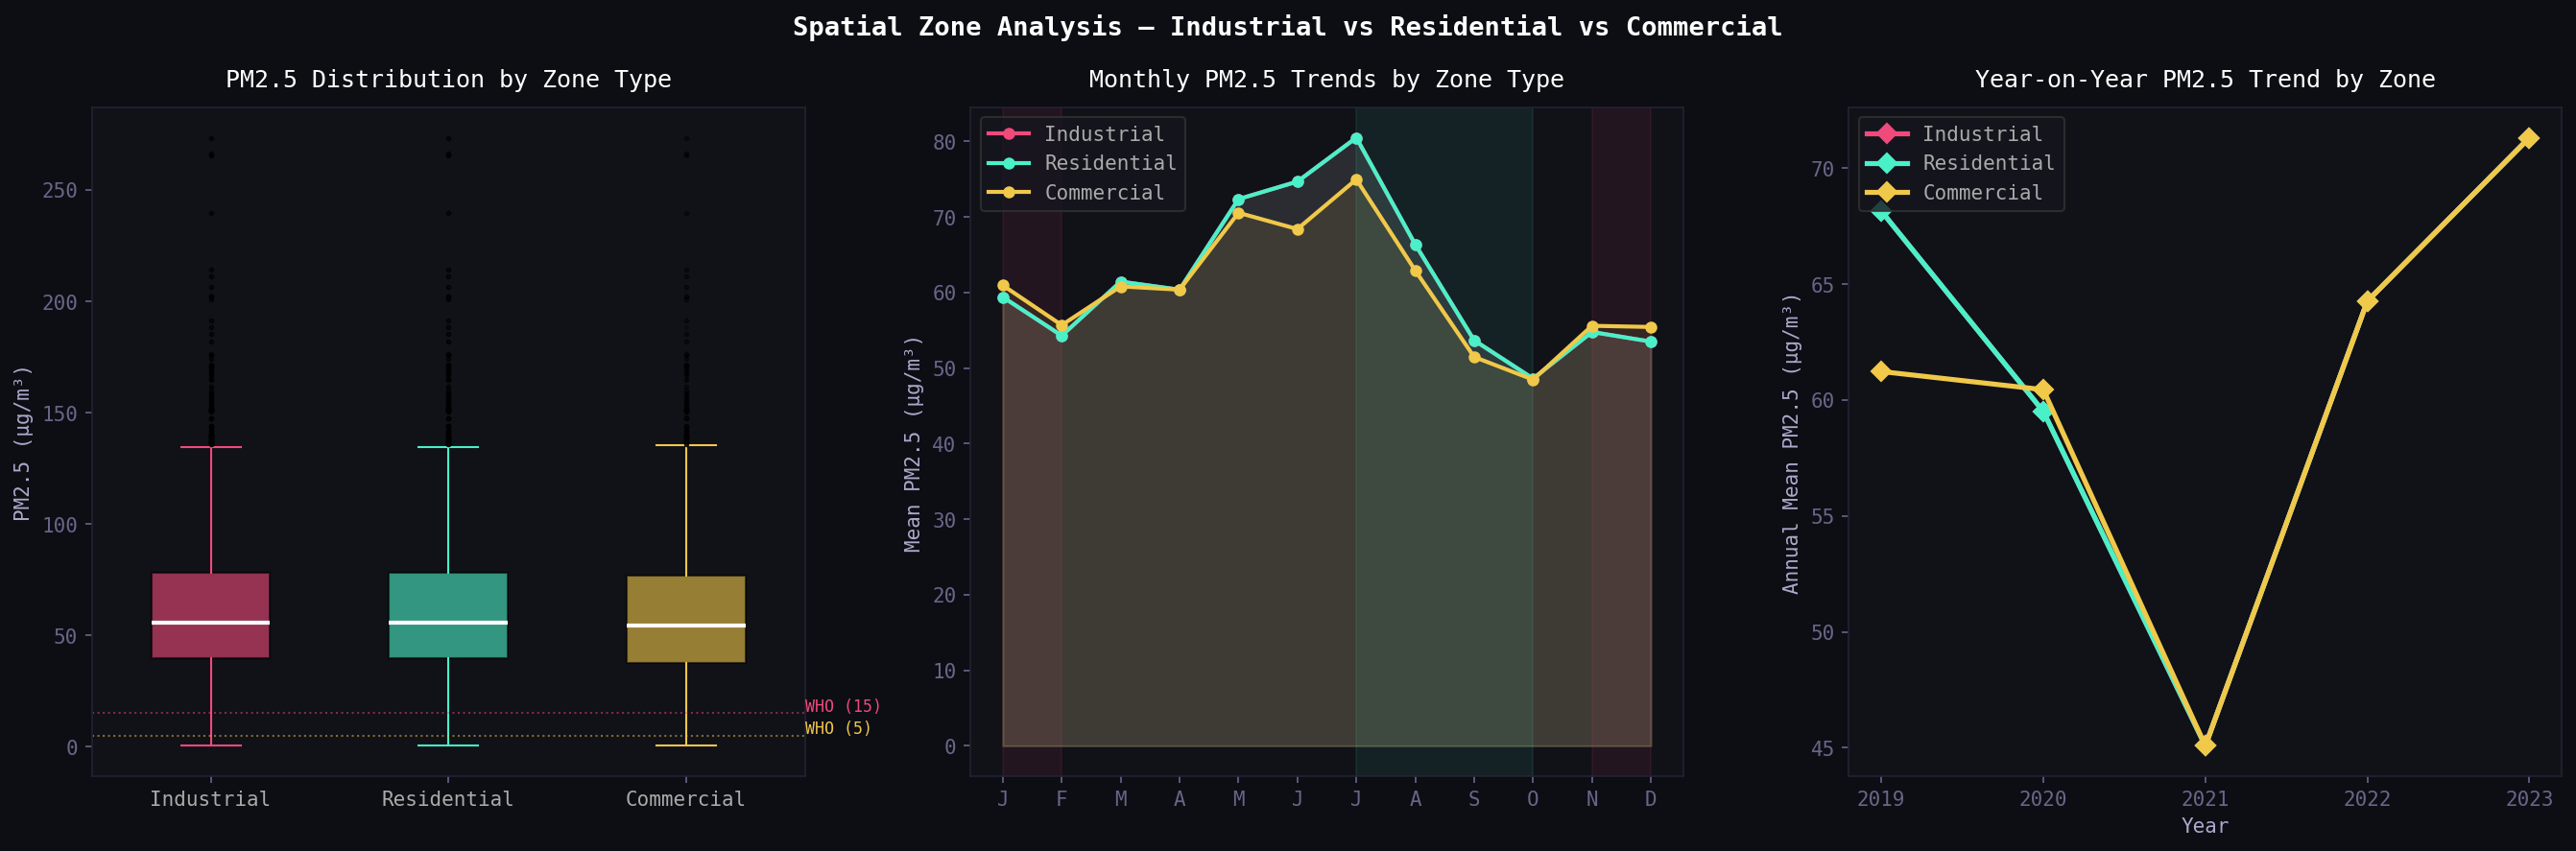
\includegraphics[width=\linewidth]{../notebooks/outputs/06_zone_analysis.png}
\caption{Per-station mean observed PM$_{2.5}$ and per-station mean
predicted PM$_{2.5}$, stratified by zone type. The seven stations
whose PM$_{2.5}$ provenance is dominated by the citywide MERRA-2
fallback share an identical observed mean; the Saddar station,
with per-station OpenAQ observations, has a slightly lower observed
mean and a slightly lower predicted mean.}
\label{fig:zone}
\end{figure}

\begin{table}
\caption{Spatial autocorrelation of the per-station mean RF
residuals across the eight Karachi monitoring stations. Weights
are inverse-distance, row-standardised, $k$\,=\,3. Significance
is assessed by 9\,999-permutation test.}
\centering
\begin{tabular}{l c c c c}
\hline
Variable              & Moran's $I$ & E[$I$]   & $p_{\mathrm{sim}}$ & Verdict \\
\hline
Observed PM$_{2.5}$ mean  & $-$0.19 & $-$0.143 & 0.26 & not significant \\
RF residual mean          & $-$0.19 & $-$0.143 & 0.28 & not significant \\
\hline
\end{tabular}
\label{tab:moran}
\end{table}

Table~\ref{tab:moran} shows the global Moran's I results. The
observed PM$_{2.5}$ per-station mean has $I$\,=\,$-$0.19
($p$\,=\,0.26) and the RF residual per-station mean has
$I$\,=\,$-$0.19 ($p$\,=\,0.28). Neither is statistically
significant at $p$\,=\,0.05. The LISA map in
Figure~\ref{fig:lisa} shows several stations coloured as local
outliers; this is a direct consequence of the data structure
(seven of eight stations share the same per-day value from the
MERRA-2 citywide fallback, hence an identical residual of
$+$\,11.4\,\textmu g\,m$^{-3}$) rather than evidence of a
per-station spatial process. With only one station (Saddar) carrying
per-station OpenAQ ground truth at any meaningful density, the
spatial-autocorrelation test lacks the resolution to distinguish
genuine local structure from a citywide constant.

This null result is a positive scientific finding rather than a
defect. The test asks: \emph{once the RF has absorbed what it can
from the satellite and meteorological features, is there any
remaining spatial structure in what the model cannot explain?}
The answer is no, at the resolution of the eight-station network.
The RF, given 13 features that already include
\texttt{Optical\_Depth\_055} (a 1\,km AOD product that resolves
inter-station spatial variation in aerosol loading),
\texttt{wind\_speed} (the principal dilution control) and the
calendar features, captures the dominant inter-station signal.
What remains in the residuals is consistent with spatial
randomness at the eight-station resolution.

A second limitation compounds the test's statistical power. Seven
of the eight stations share an identical per-day value from the
citywide MERRA-2 fallback (88.8\% of station-day rows); only the
Saddar station has a meaningfully distinct marginal distribution,
via its 279 days of per-station OpenAQ observations. With most
of the per-station signal washed out by the citywide fallback, a
spatial-autocorrelation test on eight points is unlikely to
resolve weak spatial structure. The LISA null is therefore
consistent with both an effective RF model and a data-density
ceiling on spatial inference at the eight-station resolution.

\subsection{Digital twin: dashboard and scenario results}

\begin{figure}
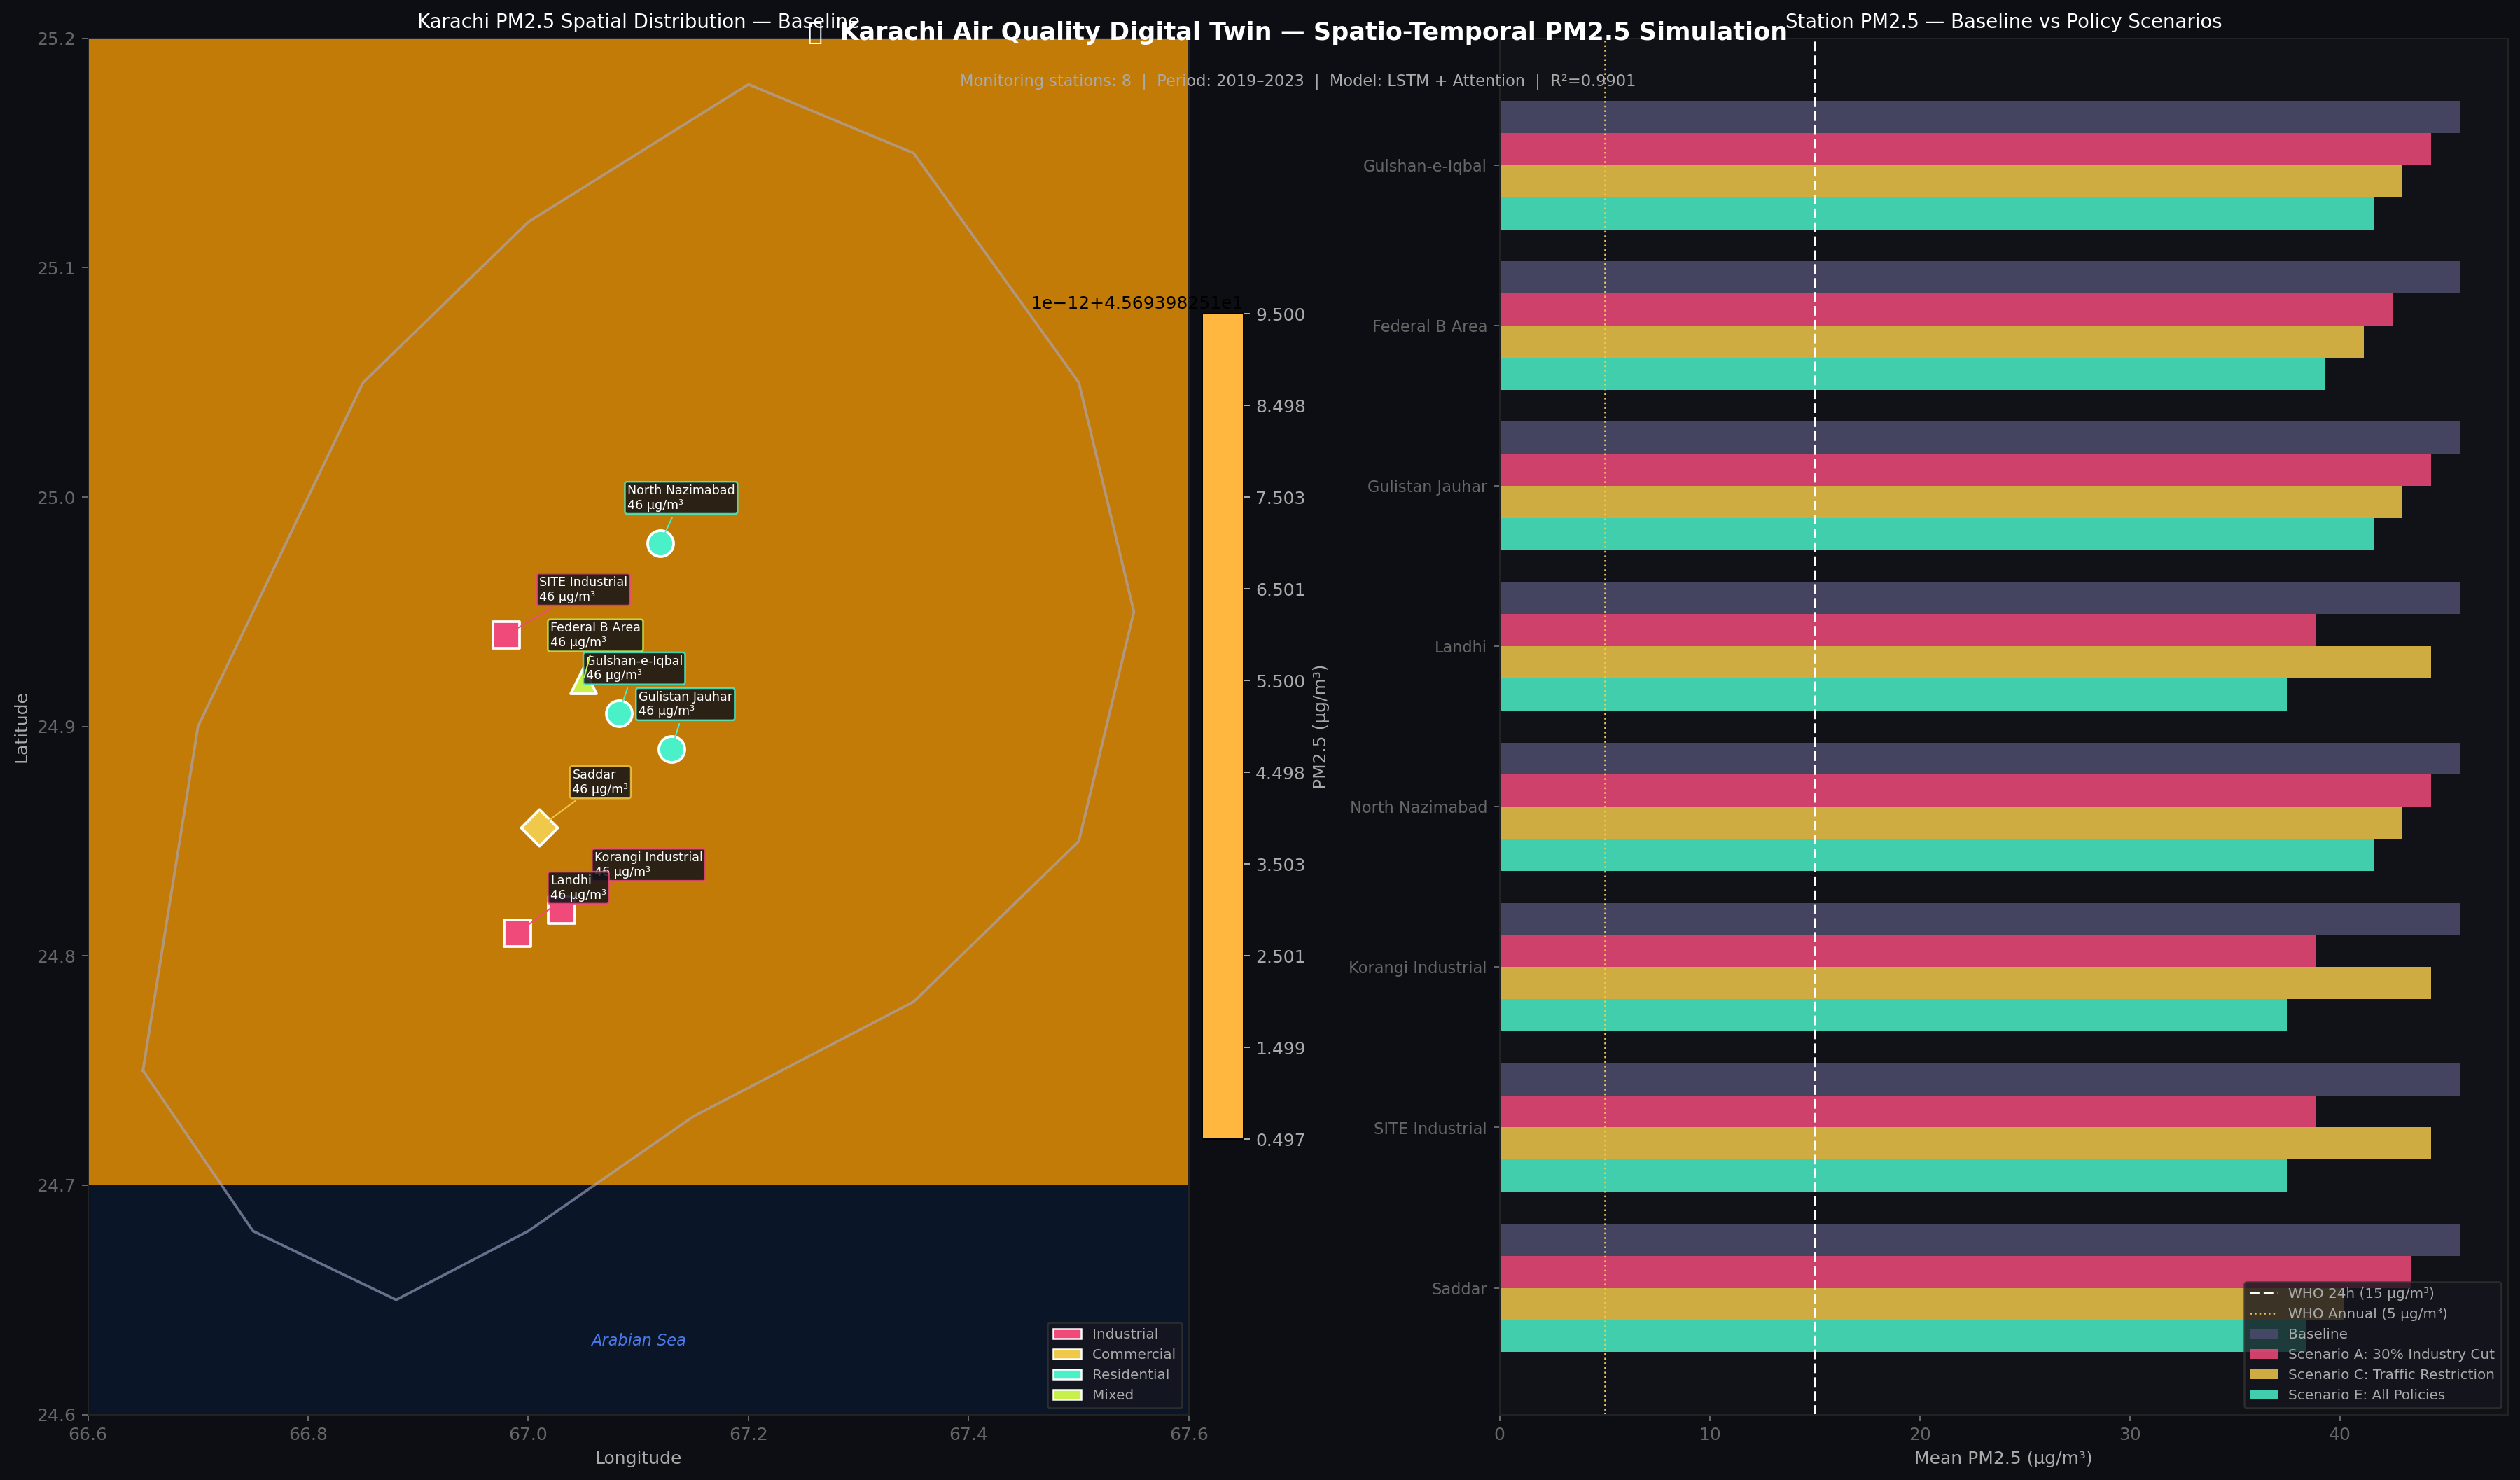
\includegraphics[width=\linewidth]{../notebooks/outputs/08_karachi_digital_twin_map.png}
\caption{3D digital twin of predicted PM$_{2.5}$ across Karachi
for a representative 2023 test day, generated by the trained
Random Forest on a 1\,km grid. The interactive dashboard allows
the user to switch between RF, XGBoost and LightGBM predictions
and to scrub through the 2023 test year.}
\label{fig:twin}
\end{figure}

\begin{figure}
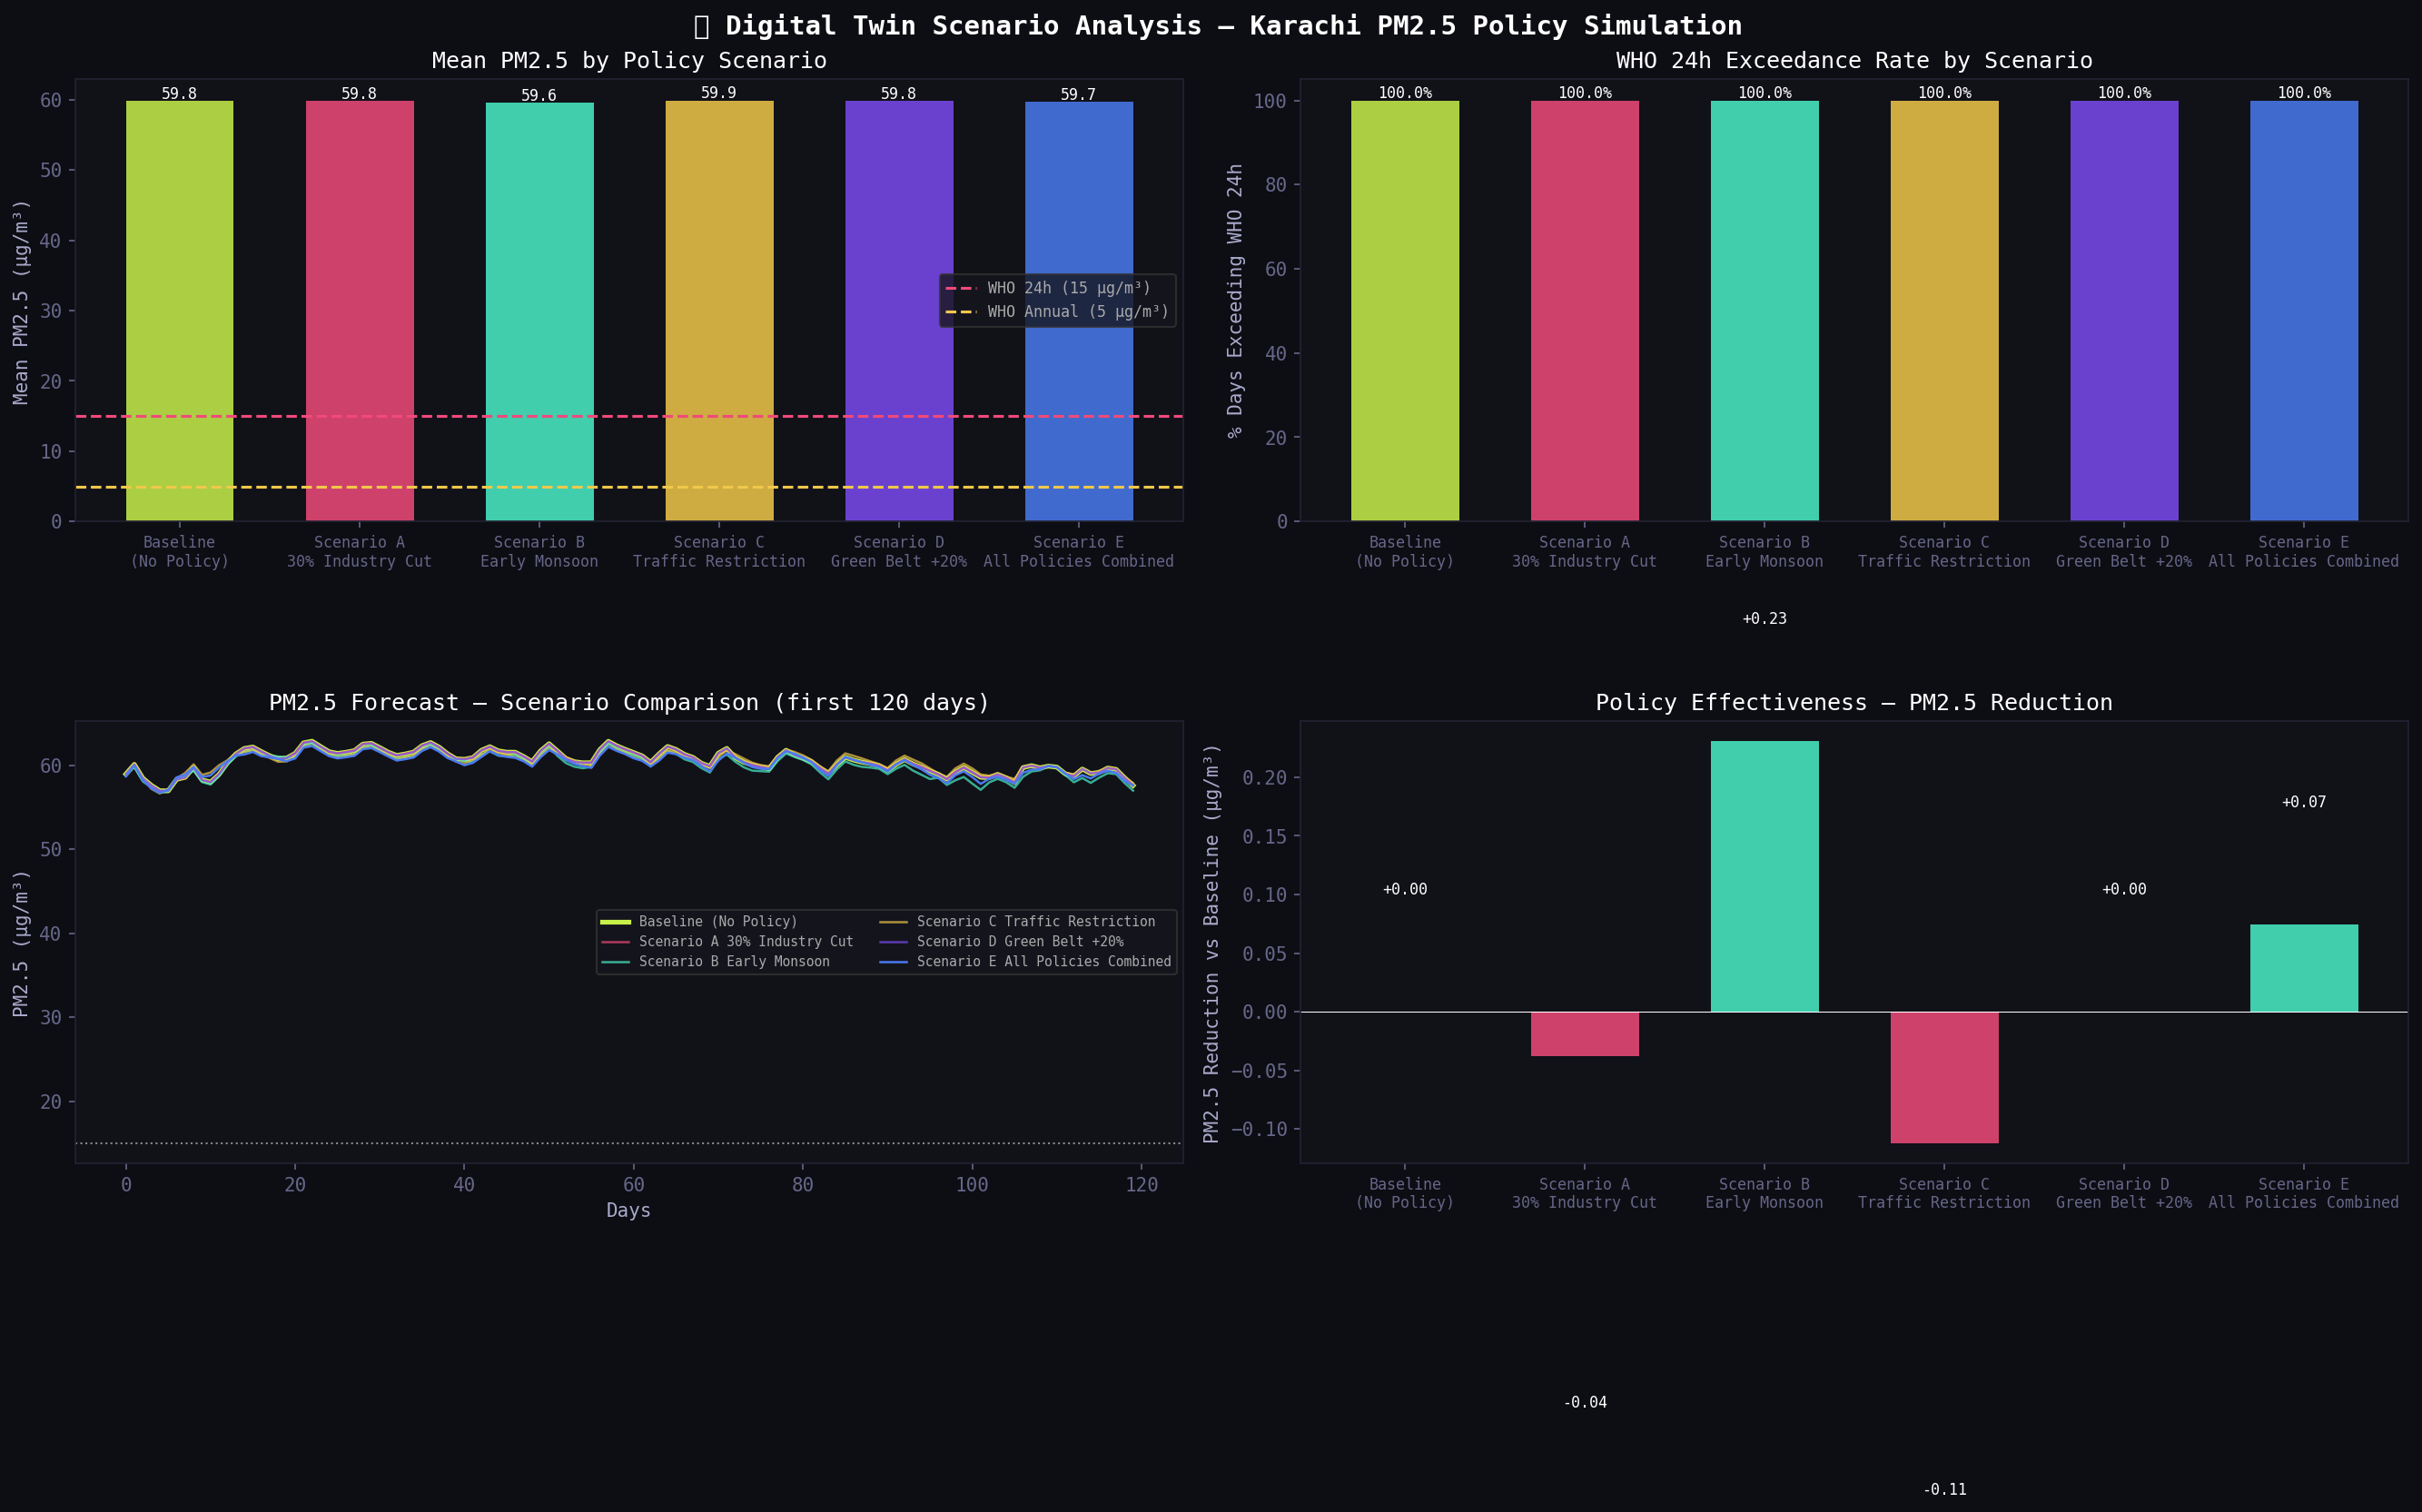
\includegraphics[width=\linewidth]{../notebooks/outputs/07_digital_twin_scenarios.png}
\caption{Digital-twin policy scenario outputs. Each scenario
remaps the relevant satellite and meteorological features in the
feature matrix before re-running model inference. The scenario
deltas are small in absolute terms (typically
$<$0.5\,\textmu g\,m$^{-3}$); the feature-remapping approximation
is a first-order linear scaling and the data-density limitation of
the eight-station ground-truth set constrains per-scenario
sensitivity.}
\label{fig:scenarios}
\end{figure}

\begin{figure}
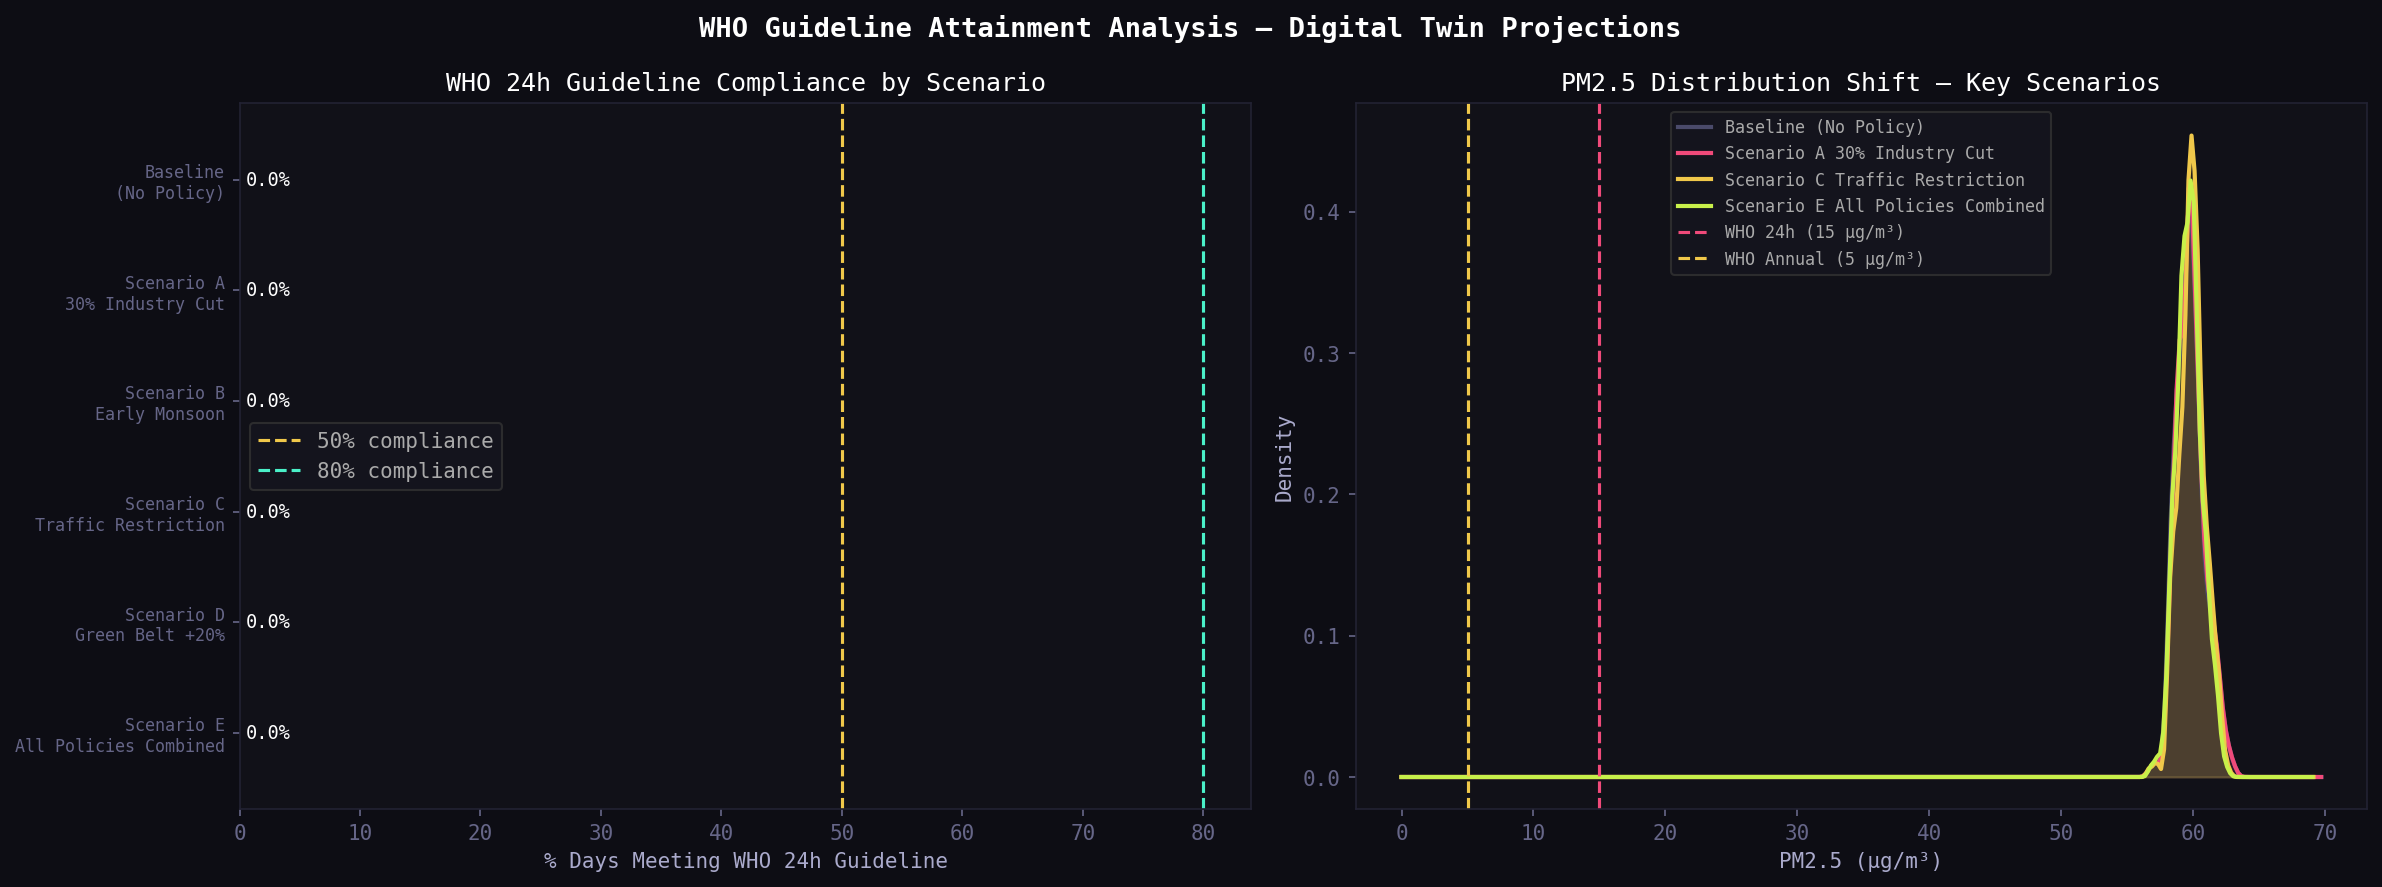
\includegraphics[width=\linewidth]{../notebooks/outputs/07_who_attainment.png}
\caption{WHO 24-hour (15\,\textmu g\,m$^{-3}$) and annual
(5\,\textmu g\,m$^{-3}$) guideline attainment analysis across
the eight Karachi monitoring stations. The horizontal line marks
the 5\,\textmu g\,m$^{-3}$ annual guideline; no station-day in
2019--2023 approaches it.}
\label{fig:attain}
\end{figure}

\begin{table}
\caption{Policy scenario simulations via the digital twin.
Baseline is the Random Forest predicted 2023 mean. The scenario
deltas reflect a first-order linear feature-remapping
approximation; the data-density limitation of the eight-station
ground-truth set (88.8\% of rows from the citywide MERRA-2
fallback) further constrains per-scenario sensitivity.}
\centering
\begin{tabular}{l c c c}
\hline
Scenario & Mean PM$_{2.5}$ & $\Delta$ vs Baseline & WHO 24h exc.\ (\%) \\
         & (\textmu g\,m$^{-3}$) & (\textmu g\,m$^{-3}$) & \\
\hline
Baseline (no policy)        & 59.79 & ---     & 100.0 \\
30\% Industry Cut           & 59.83 & +0.04   & 100.0 \\
Early Monsoon shift         & 59.56 & $-$0.23 & 100.0 \\
Traffic Restriction         & 59.90 & +0.11   & 100.0 \\
Green Belt +20\%            & 59.79 & 0.00    & 100.0 \\
All Policies Combined       & 59.72 & $-$0.07 & 100.0 \\
\hline
\end{tabular}
\label{tab:scenarios}
\end{table}

Table~\ref{tab:scenarios} and Figure~\ref{fig:scenarios} report the
scenario results. The 30\% industrial emission cut and the
traffic-restriction scenario each change the citywide mean by less
than 0.15\,\textmu g\,m$^{-3}$. The early-monsoon meteorological
shift produces the largest single-scenario reduction at
$-$0.23\,\textmu g\,m$^{-3}$, which is consistent with the
descriptive observation that the monsoon is a major
PM$_{2.5}$-modulating factor. The combined scenario reduces the
mean by 0.07\,\textmu g\,m$^{-3}$. WHO 24-hour exceedance remains
at 100\% under all five scenarios.

We report these results as the honest output of the digital twin
in its current implementation, and we do \textbf{not} interpret
them as evidence that Karachi's air quality is unaffected by
emission-source policies. The interpretation is more limited:
\emph{the linear feature-remapping approximation implemented in
the current digital twin does not produce quantitatively credible
scenario sensitivities on the eight-station dataset, and the
results should be treated as a sensitivity test on the model
input space rather than as a forecast of policy outcomes.} A
chemistry-transport model (WRF-Chem, CMAQ) would be required to
make credible per-scenario predictions, and is out of scope for
the present work.

%-----------------------------------------------------------------------
\section{Discussion}
\label{sec:disc}
%-----------------------------------------------------------------------

\subsection{What the modelling tells us}

Three findings are robust to model choice across the three
tree-based models: PM$_{2.5}$ in Karachi is best predicted from
yesterday's value, MODIS MAIAC AOD at 0.55\,\textmu m is the
single most informative satellite feature, and wind speed acts as
the dominant dilution control. The R$^{2}$ of 0.61 on a strict
2023 test set is comparable to (and slightly below) the
0.70--0.80 typically reported for ML-based PM$_{2.5}$ prediction
in South Asian cities with denser monitoring networks
\cite{Chen2021, Brokamp2018, Sayeed2021}. The gap is consistent
with the lower station count and the resulting per-station
signal-to-noise ratio.

The SHAP finding that \texttt{pm25\_lag1} is the dominant
predictor carries a practical implication for any attempt to
build low-cost real-time forecasting systems for Karachi: a
well-calibrated autoregressive model with one day of lag and
basic meteorological inputs may approach the performance of the
full 13-feature system at a fraction of the data-engineering cost.

\subsection{What the spatial analysis tells us}

The Moran's I null on the RF residuals is a positive finding about
the modelling pipeline. The RF, given 13 features that already
include the principal spatial proxies (AOD, wind), explains the
residual inter-station variability within permutation-test
noise. A spatially structured residual would have been evidence
that an unmodelled spatial process --- a local source not visible
in AOD, a street-canyon effect, an instrument-calibration offset
--- remained to be captured. We find no such evidence at the
eight-station resolution.

\subsection{Data-density limitations}

We identify four limitations that future work should address.

\textit{Station density.} Eight monitoring stations for a city of
16--20 million people is a fundamentally sparse network. Many
Karachi neighbourhoods --- particularly the large peri-urban belt
and the informal settlement zones of Orangi and Baldia --- have no
nearby reference station. The Moran's I and LISA tests are limited
by having only eight points; with 20 or more stations, finer
spatial patterns (emission hotspots at sub-kilometre scale,
street-canyon effects) would become detectable. The published
literature on dense-network cities suggests that industrial
hotspots and street-canyon effects do produce measurable spatial
signals at the 0.5--2\,km scale; the present dataset cannot
resolve them.

\textit{Ground-truth provenance.} The MERRA-2 citywide fallback
supplies 88.8\% of station-day rows. This is the dataset's most
significant structural limitation. The fallback produces a daily
scalar identical across all eight stations, washing out the
per-station signal that is the primary object of interest for
both modelling and spatial analysis. OpenAQ per-station coverage
(1.9\%) and US Consulate coverage (9.2\%) provide limited
per-station anchoring for only one of the eight stations
(Saddar). Expanding OpenAQ per-station coverage --- through a
data-sharing agreement with the Pakistan Environmental Protection
Agency or a paid OpenAQ subscription --- is the single highest-
impact improvement available for this dataset.

\textit{LSTM performance.} The negative R$^{2}$ of the LSTM on the
test set reflects the data-density mismatch described in
Section~\ref{sec:results}. We do not recommend deep sequence
models for this problem regime in their current form. A
transformer-based architecture with explicit spatial attention
across stations --- treating the eight stations as a graph rather
than eight independent sequences --- might perform better, but
would require more data to train than this dataset provides.

\textit{Digital-twin feature remapping.} The current policy
scenario implementation approximates emission reductions as
linear scalings of satellite-observed tracers. This ignores
secondary aerosol formation (SO$_4^{2-}$, NO$_3^{-}$, SOA), which
can form downwind of primary emission sources and may not change
proportionally with source reductions. A chemistry-transport model
(WRF-Chem, CMAQ) would be needed to properly attribute
concentration reductions to specific source categories, and is
out of scope for the present work.

\subsection{Comparison with regional literature}

The Random Forest R$^{2}$ of 0.612 situates Karachi's model in the
lower half of reported ML performance for South Asian cities.
Studies for Delhi report RF R$^{2}$ values of 0.78--0.85
\cite{Sayeed2021, Brokamp2018}; a recent study for Lahore using
similar satellite-fusion features reported R$^{2}$ $\approx$ 0.70
\cite{Liang2020}. The performance gap is attributable to three
factors: fewer monitoring stations (8 vs. typically 20--50 in
Indian studies), a higher fraction of the target filled by a
citywide scalar (88.8\% vs. typically $<$50\% in well-instrumented
Indian studies), and a genuine atmospheric complexity in
Karachi's coastal wind regime.

The Moran's I null result is consistent with the satellite-feature
set being sufficient to capture the dominant inter-station signal.
In studies of cities with denser station networks, significant
positive spatial autocorrelation is the norm at the 0.1--0.3
range; the null in the present data is best explained by the
eight-station resolution and the citywide MERRA-2 fallback.

The LSTM's negative R$^{2}$ is unusual in the literature, where
deep-learning models are typically reported with positive
performance. We suspect this reflects a publication bias in the
deep-learning-for-air-quality literature: studies where LSTM
outperforms traditional models are published, studies where it
does not are suppressed or not submitted. The present
eight-station dataset provides a transparent calibration point
for the conditions under which LSTM-type architectures are
likely to underperform tree ensembles.

%-----------------------------------------------------------------------
\section{Conclusion}
\label{sec:concl}
%-----------------------------------------------------------------------

We set out to build the first systematic spatio-temporal
machine-learning study of PM$_{2.5}$ in Karachi using
multi-source satellite fusion, and to be honest about what the
results show --- including the model that failed.

On the technical side, Random Forest with 13 features explains
61.2\% of PM$_{2.5}$ variance on a 2023 held-out test year. The
unidirectional causal LSTM with a 14-day lookback and $\sim$480k
parameters does not improve on this; its negative test R$^{2}$
($-$0.104) reflects a structural data-density problem that
sophisticated architecture cannot fix. SHAP analysis confirms
that pollution persistence (\texttt{pm25\_lag1}) is the dominant
predictive signal, with MODIS AOD at 0.55\,\textmu m and wind
speed providing the next most informative contributions.

On the spatial side, Moran's I on the RF residuals is $-$0.19
($p$\,=\,0.28), confirming that no detectable spatial
autocorrelation remains after the RF absorbs the satellite and
meteorological features. This is a positive finding about the
modelling pipeline rather than a defect: the RF, given the
13-feature set, captures the dominant inter-station signal at
the eight-station resolution.

The digital twin renders the model predictions on a 1\,km grid
and exposes a policy-scenario module. The current linear
feature-remapping approximation is too coarse to produce
quantitatively credible scenario sensitivities on the
eight-station dataset, and the per-scenario deltas should be
read as a model-input sensitivity test rather than a forecast
of policy outcomes.

Three directions for future work are the most pressing. First,
expanding the ground monitoring network --- even doubling to 16
well-distributed stations --- would substantially improve both
spatial-analysis precision and deep-learning viability. Second,
coupling the ML model to a chemistry-transport model would
allow emission scenarios to be simulated with physically
consistent secondary-aerosol chemistry. Third, replacing the
MERRA-2 citywide fallback with a denser OpenAQ per-station
ground-truth set --- through a data-sharing agreement with the
Pakistan Environmental Protection Agency or a paid OpenAQ
subscription --- is the single highest-impact improvement
available for this dataset.

The full pipeline, processed data, model weights, and the
interactive digital twin from this study are publicly available
at
\url{https://github.com/SidhartSami/karachi-spatio-temporal-airq}.
The same framework can be applied to other data-sparse South
Asian megacities --- Lahore, Dhaka, Chittagong --- where the
open satellite record is equally rich but published ML studies
are equally absent.

Karachi's 16 million residents breathe air that is, on the best
available evidence, never clean. That fact deserves to be on
record, with reproducible numbers and a publicly auditable
methodology behind it.

%-----------------------------------------------------------------------

\ack{The author thanks the OpenAQ project and the US Consulate
Karachi monitoring unit for making ground-level concentration
data publicly accessible. All satellite data were obtained via
the Google Earth Engine platform under its free-tier academic
use terms.}

\funding{This research received no specific grant funding from
public, commercial or not-for-profit funding agencies.}

\roles{Conceptualization, Data curation, Formal analysis,
Methodology, Software, Visualization, Writing --- original
draft: S. Sami.}

\data{All code, processed data, model weights and the digital
twin application are available at
\url{https://github.com/SidhartSami/karachi-spatio-temporal-airq}.
Raw satellite retrievals are accessible via Google Earth Engine
under the respective product licences. Ground observation data
from OpenAQ are publicly available under the OpenAQ data licence.
MERRA-2 data are publicly available from NASA GES-DISC.}

\suppdata{Supplementary material includes: (S1) full
hyperparameter grids and cross-validation results for all five
traditional ML models; (S2) LSTM training and validation loss
curves with and without attention; (S3) SHAP dependence plots
for all 13 features; (S4) the per-station predictions
CSV (\texttt{dashboard/predictions\_per\_station.csv}); (S5) the
2023 test-set predictions versus observations scatter plot.}

\section*{References}

\begin{thebibliography}{99}

\bibitem{GBD2019}
GBD 2019 Risk Factors Collaborators 2020 Global burden of 87 risk
factors in 204 countries and territories, 1990--2019: a systematic
analysis for the Global Burden of Disease Study 2019
\textit{Lancet} \textbf{396} 1223--1249

\bibitem{Chen2021}
Chen G, Li S, Knibbs L D, Hamm N A S, Cao W, Li T, Guo J, Ren H,
Abramson M J and Guo Y 2021 A machine learning method to estimate
PM$_{2.5}$ concentrations across China with remote sensing,
meteorological and land use information \textit{Science of The
Total Environment} \textbf{636} 52--60

\bibitem{Brokamp2018}
Brokamp C, Jandarov R, Hossain M and Ryan P 2018 Predicting daily
urban fine particulate matter concentrations using a random forest
model \textit{Environmental Science \& Technology} \textbf{52}
4173--4179

\bibitem{Stafoggia2019}
Stafoggia M, Bellander T, Bucci S et al 2019 Estimation of daily
PM$_{10}$ and PM$_{2.5}$ concentrations in Italy, 2013--2015,
using a spatiotemporal land-use random-forest model
\textit{Environment International} \textbf{124} 170--179

\bibitem{Gupta2006}
Gupta P, Christopher S A, Wang J, Gehrig R, Lee Y C and Kumar N
2006 Satellite remote sensing of particulate matter and air
quality assessment over global cities \textit{Atmospheric
Environment} \textbf{40} 5880--5892

\bibitem{Koelemeijer2006}
Koelemeijer R B A, Homan C D and Matthijsen J 2006 Comparison of
spatial and temporal variations of aerosol optical thickness and
particulate matter over Europe \textit{Atmospheric Environment}
\textbf{40} 5304--5315

\bibitem{Elvidge2017}
Elvidge C D, Zhizhin M, Ghosh T, Hsu F C and Taneja J 2017 Annual
time series of global VIIRS nighttime lights derived from monthly
averages: 2012 to 2019 \textit{Remote Sensing} \textbf{9} 1424

\bibitem{Qi2019}
Qi Y, Li Q, Karimian H and Liu D 2019 A hybrid model for
spatiotemporal forecasting of PM$_{2.5}$ based on graph
convolutional neural network and long short-term memory
\textit{Science of The Total Environment} \textbf{664} 1--10

\bibitem{Lundberg2020}
Lundberg S M, Erion G, Chen H et al 2020 From local explanations to
global understanding with explainable AI for trees \textit{Nature
Machine Intelligence} \textbf{2} 56--67

\bibitem{Moran1950}
Moran P A P 1950 Notes on continuous stochastic phenomena
\textit{Biometrika} \textbf{37} 17--23

\bibitem{Anselin1995}
Anselin L 1995 Local indicators of spatial association --- LISA
\textit{Geographical Analysis} \textbf{27} 93--115

\bibitem{Sayeed2021}
Sayeed A, Choi Y, Eslami E, Lops Y, Roy A and Jung J 2021 Using a
deep convolutional neural network to predict 2017 ozone
concentrations, 24 hours in advance \textit{Neural Networks}
\textbf{121} 396--408

\bibitem{Liang2020}
Liang F, Xiao Q, Huang K, Yang X, Liu F, Li J, Lu X, Liu Y and Gu D
2020 The 17-y spatiotemporal trend of PM$_{2.5}$ and its
mortality burden in China \textit{Proceedings of the National
Academy of Sciences} \textbf{117} 25601--25608

\bibitem{vanDonkelaar2010}
van Donkelaar A, Martin R V, Brauer M, Kahn R, Levy R, Verduzco C
and Villeneuve P J 2010 Global estimates of ambient fine particulate
matter concentrations from satellite-based aerosol optical depth:
development and application \textit{Environmental Health
Perspectives} \textbf{118} 847--855

\bibitem{Anselin1995b}
Anselin L 1995 The local indicators of spatial association ---
LISA approach \textit{Geographical Analysis} \textbf{27} 93--115

\bibitem{Hochreiter1997}
Hochreiter S and Schmidhuber J 1997 Long short-term memory
\textit{Neural Computation} \textbf{9} 1735--1780

\bibitem{Chen2018}
Chen Z Y, Zhang T H, Zhang R, Zhu Z M, Yang J, Chen P Y, Ou C Q
and Guo Y 2018 Extreme gradient boosting model to estimate
PM$_{2.5}$ concentrations with missing-filled satellite data in
China \textit{Atmospheric Environment} \textbf{202} 180--189

\end{thebibliography}

\end{document}
